\chapter{线性算子}
\label{chap:linear-operators}

把一个函数投影到多项式子空间，用一个核对它加权积分，或者对它求导，得到的都不再是一个数，而是另一个函数。第~\ref{chap:linear-functionals}章研究的泛函把函数压成一个读数；现在输入是函数，输出也是函数。

第~\ref{chap:functions-as-vectors}章把函数看成一个很长的向量$[\ldots,f(x),\ldots]$，每个输入$x$占一个分量。沿着这个类比再走一步：向量到向量的线性变换是矩阵，函数到函数的线性变换就是“无限维的矩阵”，称为线性算子。

矩阵作用于向量时，输出的第$i$个分量等于第$i$行与输入对应相乘再相加。把下标$i,j$换成位置$x,y$，把求和换成积分，就得到函数空间中最常见的算子：
\begin{equation}
 (\bm Kf)_i=\sum_jK_{ij}f_j
 \quad\longleftrightarrow\quad
 (Tf)(x)=\int k(x,y)f(y)\,\mathrm d\nu(y).
 \label{eq:lop-matrix-integral}
\end{equation}
这里的$k(x,y)$就是矩阵元素：$x$是行号，$y$是列号。它称为积分核，表~\ref{tab:lop-dictionary}列出本章沿用的对应关系。

\begin{BookInlineTable}
  \centering
  \caption{矩阵与线性算子的对应，以及类比需要修正的地方。}
  \label{tab:lop-dictionary}
  \begin{tabular}{lll}
    \toprule
    有限维矩阵 & 函数空间中的算子 & 需要修正之处\\
    \midrule
    矩阵元素$K_{ij}$ & 核$k(x,y)$ & 恒等与求导没有函数形式的核\\
    $\sum_jK_{ij}f_j$ & $\int k(x,y)f(y)\,\mathrm d\nu(y)$ & 积分可能发散\\
    作用于所有向量 & 定义域$D(T)$ & 求导只作用于可导函数\\
    最大放大倍数 & 算子范数$\lVert T\rVert$ & 可以是无穷\\
    共轭转置$\bm K^*$ & 伴随算子$T^*$ & 像未必是闭集\\
    低秩近似 & 有限秩逼近 & 只有紧算子能这样逼近\\
    \bottomrule
  \end{tabular}
\end{BookInlineTable}

有限维的经验在三个地方不再成立。积分可能发散，所以要写明算子作用于哪些输入。放大倍数可能没有上界，所以同一个公式换一个范数，结论就可能相反。输入、输出空间的完备性也开始起作用，一些矩阵论中理所当然的事情，如今要靠完备性才成立。

本章前四节建立算子的基本量度。第~\ref{sec:lop-definition}节规定输入、输出，并列出投影、乘法、积分与求导等例子。第~\ref{sec:lop-operator-norm}节定义有界性与算子范数，也就是矩阵的最大放大倍数。第~\ref{sec:lop-inclusions}节把“同一个函数放进不同空间”看成算子，第~\ref{sec:lop-operator-convergence}节比较算子列的两种收敛。

后三节研究矩阵论中其他结构的对应物。第~\ref{sec:lop-adjoint}节定义伴随，它是共轭转置的推广。第~\ref{sec:lop-compact}节研究能用低秩矩阵逼近的算子，即紧算子。第~\ref{sec:lop-fundamental-theorems}节在完备空间中建立一致有界原理、开映射定理与闭图判别。

本章只建立算子本身的结构。算子减去数乘恒等算子后能否稳定求逆、紧自伴算子的特征展开和奇异分解属于第~\ref{chap:operator-spectra}章；给定输出求解算子方程的可解性与稳定性属于第~\ref{chap:linear-operator-equations}章。

\section{算子的定义}
\label{sec:lop-definition}

在$L^2(0,1)$中把函数投影到常数子空间，得到它的平均值组成的常函数。对连续函数$f$作积分$x\mapsto\int_0^xf(t)\,\mathrm dt$，得到一个可导函数。对可导函数求导，又回到一个可能不再可导的函数。

三种操作的共同点是：输入一个函数，输出另一个函数，并且保持线性组合。差别在于它们对输入的要求：投影和积分对空间中每个元素都有意义，求导只对一部分函数有意义。矩阵不会遇到这种差别，算子却必须从这里说起。

\subsection{线性算子}
\label{sec:lop-linear-operators}

矩阵$\bm A\in\mathbb R^{m\times n}$作用于每个$\bm x\in\mathbb R^n$，输入、输出的所在空间由矩阵形状直接给出。函数空间中，作用规则往往先以公式出现，例如“求导”或“对核积分”，而公式本身并不说明对哪些函数有意义。因此定义算子时，要把允许的输入集合与输出所在的空间作为算子的一部分写出来。

\begin{definition}[线性算子]
\label{def:lop-linear-operator}
设$X,Y$是同一标量域$\mathbb F$（$\mathbb R$或$\mathbb C$）上的线性空间，$D(T)\subseteq X$是线性子空间。映射$T:D(T)\to Y$若满足
\begin{equation}
 T(\alpha x+\beta z)=\alpha Tx+\beta Tz\qquad(x,z\in D(T),\ \alpha,\beta\in\mathbb F),
 \label{eq:lop-linearity}
\end{equation}
则称$T$为从$X$到$Y$的\term{线性算子}（linear operator）。$D(T)$称为$T$的\term{定义域}（domain），$Y$称为它的取值空间。集合
\begin{equation}
 \operatorname{Ran}T=\{Tx:x\in D(T)\},\qquad\ker T=\{x\in D(T):Tx=0\}
 \label{eq:lop-range-null}
\end{equation}
分别称为$T$的\term{像空间}（image space）和\term{零空间}（null space），也简称像与核。
\end{definition}

定义要求$D(T)$是线性子空间，这样$\alpha x+\beta z$仍是允许的输入，线性条件才有意义。由线性得$T0=0$。像与零空间都是线性子空间：两个输出的线性组合是相应输入线性组合的输出，两个被送到零的输入之和也被送到零。

矩阵的列空间与零空间在这里仍然对应。取值空间$Y$是事先指定的，像$\operatorname{Ran}T$则由算子实际产生，二者相等时才称$T$为满射。

零空间描述哪些输入的差别在输出中完全看不见：
\[
 Tx=Tz\quad\Longleftrightarrow\quad x-z\in\ker T.
\]
所以$T$是单射当且仅当$\ker T=\{0\}$。这与矩阵情形相同，只是这里的“输入”可能是函数的等价类，零空间也要在相应意义下理解。

有限维中的秩—零化度公式却没有对应物。方阵是单射当且仅当是满射；无限维中二者彼此独立，第~\ref{sec:lop-adjoint}节的右移算子是单射但不是满射。

$D(T)=X$时，称$T$定义在整个$X$上，简记$T:X\to Y$；本章若不特别写出定义域，算子都是这种情形。另一种情形是$D(T)$只是$X$的真子空间，求导就是典型。把它看成从$C[0,1]$到$C[0,1]$的算子时，只有可导函数才是允许的输入。

两种情形必须分开：后面讨论有界性时，定义域上的范数与取值空间上的范数各自指定，而定义在真子空间上的算子是否有界，取决于在这个子空间上用什么范数衡量输入。

取值空间为标量域$\mathbb F$时，线性算子就是第~\ref{chap:linear-functionals}章的线性泛函，相当于只有一行的矩阵。下面关于算子的结论都包含泛函的情形，泛函那里建立的表示和延拓工具也会在伴随与基本定理中再次用到。

\subsection{常见算子}
\label{sec:lop-common-operators}

下面几个例子在本章反复出现。对每个例子，我们写出输入空间、输出空间与作用规则，再核对线性，并说明它相当于什么样的矩阵。重点是看出“公式能写出来”与“算子已经定义好”之间还差哪些检查。

\paragraph{恒等映射与正交投影}
对任意线性空间$X$，\term{恒等算子}（identity operator）$I_Xx=x$定义在整个$X$上。线性由定义直接得到：两边都等于$\alpha x+\beta z$。它相当于单位矩阵，不同空间各有自己的恒等算子，复合时要分清$I_X$与$I_Y$。

设$H$是Hilbert空间，$M\subseteq H$是闭子空间。第~\ref{chap:function-inner-product-spaces}章说明每个$x\in H$在$M$中有唯一的最近点$P_Mx$，并且$x-P_Mx\perp M$。由此得到正交投影$P_M:H\to H$。

正交投影的线性需要验证。向量$\alpha P_Mx+\beta P_Mz$属于$M$，并且残差
\[
 \alpha x+\beta z-(\alpha P_Mx+\beta P_Mz)=\alpha(x-P_Mx)+\beta(z-P_Mz)
\]
与$M$正交。满足这两条的元素唯一，所以它就是$P_M(\alpha x+\beta z)$。

例如在$L^2(0,1)$中取$M$为常函数子空间，单位向量$1$张成$M$，于是
\[
 P_Mf=\langle1,f\rangle\cdot1=\Bigl(\int_0^1f\,\mathrm dt\Bigr)\cdot1.
\]
这个算子的“矩阵”处处等于$1$：它的核是$k(x,y)\equiv1$，每一行都把输入平均一次。

\paragraph{固定函数相乘}
设$(\Omega,\mathcal F,\mu)$是测度空间，$\varphi\in L^\infty(\mu)$，$1\leq p\leq\infty$。对$f\in L^p(\mu)$令$M_\varphi f=\varphi f$，称为\term{乘法算子}（multiplication operator）。按分量看，它把第$x$个分量乘以$\varphi(x)$，正是对角矩阵的连续版本。

下面逐项核对。若$f=g$几乎处处，则$\varphi f=\varphi g$几乎处处，所以作用对等价类有确定的意义。由几乎处处成立的不等式
\[
 \lvert\varphi f\rvert\leq\lVert\varphi\rVert_\infty\lvert f\rvert,
\]
输出仍在$L^p(\mu)$中。线性来自乘法对加法的分配律。

对角元素无界时情况就变了。在$(0,1)$上取$\varphi(x)=x^{-1}$，函数$f=1$属于$L^2(0,1)$，而$\varphi f=x^{-1}$不平方可积。公式仍可写出，却不再给出$L^2$到$L^2$的算子。

\paragraph{积分变换}
设$(X,\mu)$与$(Y,\nu)$是测度空间，$k:X\times Y\to\mathbb F$可测。形式上令
\begin{equation}
 (Tf)(x)=\int_Yk(x,y)f(y)\,\mathrm d\nu(y),\qquad x\in X,
 \label{eq:lop-integral-operator}
\end{equation}
称$k$为\term{积分核}（integral kernel），$T$为以$k$为核的\term{积分算子}（integral operator）。按式~\eqref{eq:lop-matrix-integral}的类比，第一个变量$x$是输出的位置，也就是行；第二个变量$y$是输入的位置，也就是列。固定$x$，$k(x,\cdot)$就是这一行的全部元素。

只要右端对每个输入有意义，线性就由积分的线性得到。问题在于“有意义”需要核、参考测度和输入函数共同决定。在$[0,1]$上取Lebesgue测度与核$k\equiv1$，则
\[
 (Tf)(x)=\int_0^1f(y)\,\mathrm dy.
\]
对$f(y)=y^{-1/2}$积分为$2$，对$f(y)=y^{-1}$积分发散。

保持核与输入不变，把测度换成$y\,\mathrm dy$，$f(y)=y^{-1}$的积分就变成$1$。所以积分公式本身不是算子：要先指定输入空间与测度，核对积分对几乎每个$x$绝对收敛、输出可测并落在指定的输出空间中，才得到一个算子。第~\ref{sec:lop-integral-bounded}小节将在平方可积核的条件下完成这些检查。

本章用一个具体的积分算子作贯穿例子。在$[-1,1]$上取概率测度$\mathrm d\mu(z)=\mathrm dz/2$与核$k(x,z)=1+xz$，则
\begin{equation}
 (Tf)(x)=\int_{-1}^1f\,\mathrm d\mu+x\int_{-1}^1zf(z)\,\mathrm d\mu(z).
 \label{eq:lop-running-kernel}
\end{equation}
输出总是一次函数，两个系数是输入的零阶矩与一阶矩。

取输入$f=1+x$，两个矩分别是
\[
 \int_{-1}^1(1+z)\,\mathrm d\mu=1,\qquad
 \int_{-1}^1z(1+z)\,\mathrm d\mu=\int_{-1}^1z^2\,\mathrm d\mu=\frac13.
\]
于是$Tf=1+x/3$。再取$q(x)=x^2-1/3$，它的两个矩都为零，所以$Tq=0$，$q\in\ker T$。

矩阵的类比可以真正算出来。把$[-1,1]$等分成四格，取中点作下标：
\[
 x_i\in\Bigl\{-\frac34,\ -\frac14,\ \frac14,\ \frac34\Bigr\}.
\]
每格的$\mu$测度是$1/4$，积分近似成求和，矩阵元素取核的值$K_{ij}=1+x_ix_j$：
\[
 (Tf)(x_i)\approx\frac14\sum_{j=1}^4K_{ij}f(x_j).
\]

输入取$f=1+x$，它在四个中点的值是$(1/4,\,3/4,\,5/4,\,7/4)$。第一行的矩阵元素是$(25/16,\,19/16,\,13/16,\,7/16)$，于是
\[
 (Tf)(x_1)\approx\frac14\cdot\frac{25+57+65+49}{64}=\frac{49}{64}\approx0.766.
\]
准确值是$Tf(-3/4)=1-1/4=0.75$。四个格子已经给出接近的结果，图~\ref{fig:lop-kernel-as-matrix}(a)画出了全部四行。

\begin{BookInlineFigure}
  \centering
  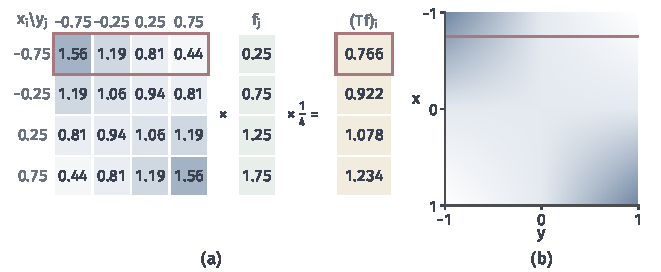
\includegraphics[width=112mm]{figures/04-spaces-measures-and-geometry/03-function-spaces/matplotlib/lop-kernel-as-matrix/figure.pdf}
  \caption{积分算子是矩阵的连续版本，核$k(x,y)=1+xy$就是矩阵元素。(a)四个中点上的矩阵$K_{ij}=1+x_ix_j$，乘以输入$f=1+x$的取值（绿）和格子测度$1/4$，得到输出的近似值（黄）；红框是第一行与它给出的输出。(b)同一个核在连续变量下的取值，纵轴向下对应行号，颜色越深值越大，红线是$x=-3/4$的一行。}
  \label{fig:lop-kernel-as-matrix}
\end{BookInlineFigure}

图中(b)是把格子无限加细后的样子。行变成水平切片，矩阵元素变成曲面上的一点，$k(x,\cdot)$作用于输入的方式与(a)中的第一行相同。

这个对应在哪里失效，也应当说清楚。恒等算子的矩阵是对角线上全为$1$。对角线$\{x=y\}$在正方形中面积为零，任何函数形式的核都承载不了它，所以恒等算子在$L^2(0,1)$上不是积分算子。求导相当于差分矩阵，同样只有对角线附近的元素，也没有函数形式的核。

\paragraph{微分}
在$[0,1]$上令$Df=f^\prime$。连续函数未必可导，例如$f(x)=\lvert x-1/2\rvert$在$x=1/2$处没有导数，所以$D$不能定义在整个$C[0,1]$上。

取定义域$D(D)=C^1[0,1]$，即导数存在且连续的函数，输出$f^\prime\in C[0,1]$，线性来自求导的线性。于是求导是一个从$C[0,1]$到$C[0,1]$、定义在真子空间$C^1[0,1]$上的线性算子。它也可以看成从$C^1[0,1]$到$C[0,1]$的算子，两种看法的区别要到配置范数时才显现出来。

这些例子中，恒等、投影与乘以有界函数自然定义在整个空间上；积分变换须由核与测度的条件保证定义；求导只能定义在一部分函数上。下一节为输入与输出配上范数，研究这些算子是否用一个统一的常数控制误差。

\section{算子范数}
\label{sec:lop-operator-norm}

输入$x$带上扰动$e$以后，线性算子的输出变为$T(x+e)=Tx+Te$。输出误差$Te$只取决于扰动本身，与$x$在哪里无关。于是“误差会被放大多少”化为一个问题：能否找到一个常数，控制一切扰动经过$T$后的大小？

对矩阵，这个问题总有答案。单位球是紧集，$\lVert\bm A\bm x\rVert$连续，最大值一定取到。算子没有这样的保证：单位球不紧，放大倍数可能无穷大。本节先用一个统一不等式定义有界性，再通过求导和积分说明条件的作用，最后定义算子范数。

\subsection{算子的有界性}
\label{sec:lop-boundedness}

下面设$X,Y$是赋范空间，$T:D(T)\to Y$是线性算子，$D(T)\subseteq X$沿用$X$的范数，$Y$使用它自己的范数。我们希望用一个与输入无关的常数$C$控制$\lVert Tx\rVert$，这样输入误差为$\lVert e\rVert$时，输出误差不超过$C\lVert e\rVert$。

\begin{definition}[有界线性算子]
\label{def:lop-bounded-operator}
若存在常数$C\geq0$，使
\begin{equation}
 \lVert Tx\rVert_Y\leq C\lVert x\rVert_X\qquad(x\in D(T)),
 \label{eq:lop-bounded}
\end{equation}
则称线性算子$T$为\term{有界线性算子}（bounded linear operator），简称有界算子。不存在这样的常数时，称$T$为\term{无界算子}（unbounded operator）。
\end{definition}

这里的“有界”说的是输出与输入之比有统一上界，不是说输出集合$\{Tx:x\in D(T)\}$有界：非零线性算子的像在数乘下封闭，总是无界集合。条件~\eqref{eq:lop-bounded}也可以只在单位球上检查。按线性把$x\neq0$缩放为$x/\lVert x\rVert$，它等价于
\[
 \sup\{\lVert Tx\rVert:x\in D(T),\ \lVert x\rVert\leq1\}<\infty.
\]

第~\ref{chap:metric-space-maps}章在度量空间之间定义了连续映射与Lipschitz映射：后者要求存在常数$L$使输出距离不超过$L$倍的输入距离，它比连续更强。对一般映射，二者相差很远；对线性算子，下面的定理说明它们与有界性是一回事。

\begin{theorem}[有界与连续等价]
\label{thm:lop-bounded-continuous}
对赋范空间之间的线性算子$T:D(T)\to Y$，下列四条等价：（i）$T$在$0$处连续；（ii）$T$在$D(T)$上处处连续；（iii）$T$是Lipschitz映射；（iv）$T$有界。
\end{theorem}

\begin{proof}
若（iv）成立，由线性，
\[
 \lVert Tx-Tz\rVert=\lVert T(x-z)\rVert\leq C\lVert x-z\rVert,
\]
这就是（iii）。Lipschitz映射处处连续，故（iii）推出（ii）；处处连续自然包含在$0$处连续，故（ii）推出（i）。

只需再证（i）推出（iv）。取$\varepsilon=1$，由$T$在$0$处连续及$T0=0$，存在$\delta>0$，使$x\in D(T)$且$\lVert x\rVert\leq\delta$时$\lVert Tx\rVert\leq1$。

对任意$x\neq0$，向量$\delta x/\lVert x\rVert$的范数为$\delta$，于是
\[
 \lVert Tx\rVert=\frac{\lVert x\rVert}{\delta}\Bigl\lVert T\Bigl(\frac{\delta x}{\lVert x\rVert}\Bigr)\Bigr\rVert\leq\frac{1}{\delta}\lVert x\rVert .
\]
取$C=1/\delta$即得（iv）。
\end{proof}

证明的关键是缩放：线性算子在零点附近一个小球上的行为，决定了它在所有尺度上的行为。有限维空间中所有范数等价，线性映射总是有界的；无限维中这一点不再自动成立，下面两个例子分别给出失败与成立的情形。

\subsubsection{有界性依赖定义域范数}
\label{sec:lop-derivative-boundedness}

求导的“矩阵”先用差分看清楚。在$[0,1]$上取$n+1$个等距点，步长$h=1/n$，差分$(f_{i+1}-f_i)/h$就是一行只有两个非零元素$\pm1/h$的矩阵。网格加细时，矩阵元素按$1/h$增大。

取输入为交错序列$f_i=(-1)^i$，它的每个分量绝对值都是$1$，输出的每个分量绝对值都是$2/h=2n$。例如$h=1/4$时，输入$(1,-1,1,-1,1)$的输出是$(-8,8,-8,8)$。网格越细，这个矩阵的放大倍数越大，极限下不存在上界。积分的矩阵正好相反，元素里带一个小因子$h$。

现在回到连续的情形。考虑求导$D:C^1[0,1]\to C[0,1]$，$Df=f^\prime$，取值空间始终使用一致范数$\lVert g\rVert_\infty=\max_{[0,1]}\lvert g\rvert$。先在定义域上使用同时计入函数值与导数的范数
\[
 \lVert f\rVert_{C^1}=\lVert f\rVert_\infty+\lVert f^\prime\rVert_\infty .
\]
这时
\[
 \lVert Df\rVert_\infty=\lVert f^\prime\rVert_\infty\leq\lVert f\rVert_{C^1},
\]
取$C=1$即满足式~\eqref{eq:lop-bounded}，$D$是有界算子。

再在同一个函数集合$C^1[0,1]$上只用一致范数衡量输入。取$f_n(x)=\sin(2\pi nx)$，则
\[
 \lVert f_n\rVert_\infty=1,\qquad \lVert Df_n\rVert_\infty=\lVert2\pi n\cos(2\pi nx)\rVert_\infty=2\pi n .
\]
输出与输入的范数之比为$2\pi n$，随$n$无界增长，不存在统一常数，$D$是无界算子。振幅不变而频率升高时，函数值始终在$[-1,1]$中，斜率却按频率放大；一个一致范数很小的高频扰动$\varepsilon f_n$，可以使导数产生$2\pi n\varepsilon$的误差。

两种情形中，求导公式与允许的函数集合都没有变，变化的只是定义域上的范数。所以说一个算子是否有界，必须同时交代作用规则、定义域和两侧的范数。前一种范数把导数的大小也算进输入的“大小”，因而能控制输出；后一种范数看不见导数，也就无从控制它。

两种范数的另一个差别是完备性。只配一致范数的$C^1[0,1]$不是Banach空间。函数$g_n(x)=\sqrt{(x-1/2)^2+n^{-2}}$都连续可导，并且
\[
 0\leq g_n(x)-\lvert x-\tfrac12\rvert=\frac{n^{-2}}{g_n(x)+\lvert x-1/2\rvert}\leq\frac1n,
\]
所以$(g_n)$按一致范数收敛到不可导的$\lvert x-1/2\rvert$，是$C^1[0,1]$中没有极限的柯西列。

第~\ref{sec:lop-fundamental-theorems}节的算子定理都要求Banach空间，因此不能直接套用在这样的定义域上。配上$\lVert\cdot\rVert_{C^1}$后，$C^1[0,1]$是完备的（第~\ref{sec:lop-closed-graph}小节用积分表示说明这一点），那些定理才能使用。

\subsubsection{积分算子的有界性}
\label{sec:lop-integral-bounded}

现在回到积分变换~\eqref{eq:lop-integral-operator}。先看矩阵的情形。输出的第$i$个分量是第$i$行与输入的内积，由Cauchy--Schwarz不等式，它的平方不超过第$i$行的平方和乘以$\lVert\bm f\rVert^2$。

再对$i$求和，就得到
\[
 \lVert\bm K\bm f\rVert^2\leq\Bigl(\sum_{i,j}\lvert K_{ij}\rvert^2\Bigr)\lVert\bm f\rVert^2.
\]
右端括号是矩阵元素的平方和，即Frobenius范数的平方。把求和换成积分，同一个估计给出下面的定理，核的$L^2$范数相当于矩阵的Frobenius范数。

设$(X,\mu)$与$(Y,\nu)$是$\sigma$有限测度空间，固定输入空间$L^2(Y,\nu)$、输出空间$L^2(X,\mu)$，并设核$k\in L^2(X\times Y,\mu\otimes\nu)$。下面用到的乘积测度、Tonelli定理与Fubini定理见第~\ref{chap:integration}章。

\begin{theorem}[平方可积核的有界性]
\label{thm:lop-hs-bounded}
在上述条件下，对每个$f\in L^2(Y,\nu)$，积分~\eqref{eq:lop-integral-operator}对$\mu$几乎每个$x$绝对收敛，所得函数$Tf$可测且属于$L^2(X,\mu)$，并且
\begin{equation}
 \lVert Tf\rVert_{L^2(X,\mu)}\leq\lVert k\rVert_{L^2(X\times Y,\mu\otimes\nu)}\lVert f\rVert_{L^2(Y,\nu)} .
 \label{eq:lop-hs-bound}
\end{equation}
因此$T:L^2(Y,\nu)\to L^2(X,\mu)$是有界线性算子。
\end{theorem}

\begin{proof}
第一步，取得平方可积的截面。对非负可测函数$\lvert k\rvert^2$用Tonelli定理，
\[
 \int_X\Bigl(\int_Y\lvert k(x,y)\rvert^2\,\mathrm d\nu(y)\Bigr)\mathrm d\mu(x)=\lVert k\rVert_{L^2(\mu\otimes\nu)}^2<\infty ,
\]
所以内层积分对$\mu$几乎每个$x$有限，即截面$k(x,\cdot)\in L^2(Y,\nu)$对几乎每个$x$成立。

第二步，逐点估计。对这样的$x$，由Cauchy--Schwarz不等式，
\[
 \int_Y\lvert k(x,y)f(y)\rvert\,\mathrm d\nu(y)\leq\lVert k(x,\cdot)\rVert_{L^2(\nu)}\lVert f\rVert_{L^2(\nu)}<\infty ,
\]
积分绝对收敛，并且
\[
 \lvert(Tf)(x)\rvert\leq\lVert k(x,\cdot)\rVert_{L^2(\nu)}\lVert f\rVert_{L^2(\nu)}.
\]
在例外的零测集上令$Tf=0$。

第三步，核对可测性。取$\mu(E)<\infty$的可测集$E\subseteq X$，对第二步的逐点界关于$x\in E$积分，再用一次Cauchy--Schwarz不等式，
\[
 \int_E\int_Y\lvert k(x,y)f(y)\rvert\,\mathrm d\nu(y)\,\mathrm d\mu(x)
 \leq\mu(E)^{1/2}\lVert k\rVert_{L^2(\mu\otimes\nu)}\lVert f\rVert_{L^2(\nu)}<\infty .
\]
所以$(x,y)\mapsto k(x,y)f(y)$在$E\times Y$上可积，由Fubini定理，内层积分$x\mapsto(Tf)(x)$在$E$上可测。$X$是可数个有限测度集合之并，故$Tf$在$X$上可测。

第四步，对$x$积分。把第二步的逐点界平方后积分，再用第一步的等式，
\[
 \begin{aligned}
 \lVert Tf\rVert_{L^2(\mu)}^2
 &\leq\int_X\lVert k(x,\cdot)\rVert_{L^2(\nu)}^2\,\mathrm d\mu(x)\,\lVert f\rVert_{L^2(\nu)}^2\\
 &=\lVert k\rVert_{L^2(\mu\otimes\nu)}^2\lVert f\rVert_{L^2(\nu)}^2 .
 \end{aligned}
\]

最后，若$f=g$几乎处处，两者的积分对每个允许的$x$相同，所以$T$作用在等价类上是确定的；线性来自积分的线性。
\end{proof}

平方可积核给出的积分算子称为\term{Hilbert--Schmidt积分算子}（Hilbert--Schmidt integral operator）。证明中的每一步都依赖所选的空间：核平方可积保证截面平方可积，输入属于$L^2(\nu)$才能与截面配对，输出的估计又是按$L^2(\mu)$范数给出的。同一个核公式换成别的输入空间，就要重新核对。

平方可积只是充分条件。取$X=Y=\mathbb N$并配计数测度，$L^2$就是$\ell^2$，积分就是求和，核就是真正的无穷矩阵。单位矩阵$k(m,n)=1$（$m=n$）、$k(m,n)=0$（$m\neq n$）给出恒等算子，它有界；但$\sum_{m,n}\lvert k(m,n)\rvert^2$是无穷多个$1$之和，发散。

\subsection{算子范数的定义}
\label{sec:lop-norm-definition}

有界性只说常数$C$存在，不同的$C$都可以满足式~\eqref{eq:lop-bounded}。为了比较不同算子放大误差的程度，我们取能够使用的最小常数。这正是矩阵的最大放大倍数在算子上的对应物。

\begin{definition}[算子范数]
\label{def:lop-operator-norm}
设$T:D(T)\to Y$是有界线性算子。称
\begin{equation}
 \lVert T\rVert=\sup\{\lVert Tx\rVert_Y:x\in D(T),\ \lVert x\rVert_X\leq1\}
 \label{eq:lop-operator-norm}
\end{equation}
为$T$的\term{算子范数}（operator norm）。
\end{definition}

\begin{theorem}[算子范数是最小的误差常数]
\label{thm:lop-norm-minimal}
设$T$有界。则对一切$x\in D(T)$，
\begin{equation}
 \lVert Tx\rVert\leq\lVert T\rVert\,\lVert x\rVert,
 \label{eq:lop-norm-inequality}
\end{equation}
并且若常数$C\geq0$满足式~\eqref{eq:lop-bounded}，则$\lVert T\rVert\leq C$。因此$\lVert T\rVert$是式~\eqref{eq:lop-bounded}中可取的最小非负常数。
\end{theorem}

\begin{proof}
对$x\neq0$，$x/\lVert x\rVert$属于单位球，由定义它的输出范数不超过$\lVert T\rVert$，乘回$\lVert x\rVert$即得第一式；$x=0$时两边都为零。

反过来，若$C$满足式~\eqref{eq:lop-bounded}，则对单位球中的每个$x$有$\lVert Tx\rVert\leq C\lVert x\rVert\leq C$，对$x$取上确界得$\lVert T\rVert\leq C$。
\end{proof}

对两个输入之差用式~\eqref{eq:lop-norm-inequality}，再由线性，得到
\begin{equation}
 \lVert Tx-Tz\rVert\leq\lVert T\rVert\,\lVert x-z\rVert\qquad(x,z\in D(T)).
 \label{eq:lop-lipschitz}
\end{equation}
所以算子范数统一控制输入差造成的输出差：无论输入落在哪里，误差至多被放大$\lVert T\rVert$倍，而且没有更小的常数对全部输入都有效。

\paragraph{求导的算子范数}
对配$\lVert\cdot\rVert_{C^1}$的求导，上一小节已得$\lVert D\rVert\leq1$。取$f_n(x)=\sin(2\pi nx)/(2\pi n)$，有
\[
 \lVert Df_n\rVert_\infty=1,\qquad\lVert f_n\rVert_{C^1}=1+\frac1{2\pi n},
\]
比值趋于$1$，所以$\lVert D\rVert=1$。这个上确界不被任何输入取到：$\lVert Df\rVert_\infty=\lVert f\rVert_{C^1}$要求$\lVert f\rVert_\infty=0$。因此算子范数应理解为最小的统一上界，不能无条件称为“最大输出”。

\paragraph{积分算子的两个范数}
对平方可积核，定理~\ref{thm:lop-hs-bounded}与定理~\ref{thm:lop-norm-minimal}合起来给出
\begin{equation}
 \lVert T\rVert\leq\lVert k\rVert_{L^2(X\times Y,\mu\otimes\nu)} .
 \label{eq:lop-hs-norm}
\end{equation}
左边相当于矩阵的最大放大倍数，右边相当于矩阵元素的平方和开根。矩阵论中这两个数一般不相等，下面用贯穿例子把两个数都算出来。

先算核的$L^2$范数。在例子~\eqref{eq:lop-running-kernel}中，$\int x\,\mathrm d\mu=0$，$\int x^2\,\mathrm d\mu=1/3$，所以
\[
 \lVert k\rVert_{L^2(\mu\otimes\mu)}^2=\iint(1+xz)^2\,\mathrm d\mu(x)\,\mathrm d\mu(z)=1+2\cdot0+\frac13\cdot\frac13=\frac{10}{9}.
\]

算子范数可以直接算出。函数$e_1=1$与$e_2=\sqrt3x$在$L^2(\mu)$中标准正交，因为$\int3x^2\,\mathrm d\mu=1$。式~\eqref{eq:lop-running-kernel}可写成
\[
 Tf=\langle e_1,f\rangle e_1+\frac13\langle e_2,f\rangle e_2.
\]
在坐标$(\langle e_1,f\rangle,\langle e_2,f\rangle)$下，$T$相当于对角矩阵$\operatorname{diag}(1,1/3)$，其余方向全部被送到零。

由勾股定理和Bessel不等式，
\[
 \lVert Tf\rVert^2=\lvert\langle e_1,f\rangle\rvert^2+\frac19\lvert\langle e_2,f\rangle\rvert^2\leq\lvert\langle e_1,f\rangle\rvert^2+\lvert\langle e_2,f\rangle\rvert^2\leq\lVert f\rVert^2 .
\]
取$f=e_1=1$时等号成立，所以$\lVert T\rVert=1$，严格小于$\sqrt{10/9}=\sqrt{10}/3$。核的$L^2$范数只是算子范数的上界，二者一般不相等。

图~\ref{fig:lop-norm-ellipse}画出这件事。单位圆被压成半轴为$1$与$1/3$的椭圆，最长半轴就是算子范数。$f=1+x$的放大倍数可以直接算出。由$\lVert e_2\rVert=1$及$f=e_1+e_2/\sqrt3$，得到
\[
 \lVert f\rVert^2=1+\frac13=\frac43,\qquad\lVert Tf\rVert^2=1+\frac19\cdot\frac13=\frac{28}{27}.
\]
两式相除，放大倍数是
\[
 \frac{\lVert Tf\rVert}{\lVert f\rVert}=\sqrt{\frac{28}{27}\cdot\frac34}=\frac{\sqrt7}3\approx0.882.
\]

\begin{BookInlineFigure}
  \centering
  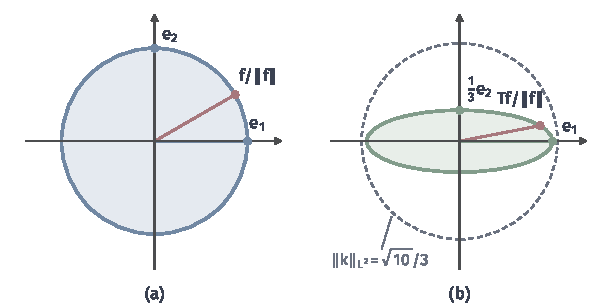
\includegraphics[width=104mm]{figures/04-spaces-measures-and-geometry/03-function-spaces/matplotlib/lop-norm-ellipse/figure.pdf}
  \caption{贯穿例子在$\operatorname{span}\{e_1,e_2\}$上的放大倍数。(a)输入坐标$(\langle e_1,f\rangle,\langle e_2,f\rangle)$中的单位圆（蓝），红点是归一化的$f=1+x$。(b)输出的椭圆（绿），半轴$1$与$1/3$，最长半轴等于$\lVert T\rVert=1$；虚线圆的半径是核的$L^2$范数$\sqrt{10}/3$，它只是上界。}
  \label{fig:lop-norm-ellipse}
\end{BookInlineFigure}

\paragraph{有界算子的矩阵}
到目前为止，矩阵只是类比。在可分Hilbert空间中，有界性让这个类比成为等式。设$H$有标准正交基$(e_n)_{n\geq1}$，$T\in\mathcal B(H)$（记号见下一小节），规定矩阵元素
\begin{equation}
 A_{mn}=\langle e_m,Te_n\rangle .
 \label{eq:lop-matrix-entry}
\end{equation}

任取$x=\sum_nx_ne_n$，部分和$\sum_{n\leq N}x_ne_n$按范数收敛到$x$。由$T$连续，
\[
 Tx=\lim_{N\to\infty}\sum_{n\leq N}x_nTe_n.
\]
再用内积对第二个变量连续，读出第$m$个坐标，就得到矩阵乘法公式
\[
 \langle e_m,Tx\rangle=\sum_nA_{mn}x_n .
\]
连续性在这里不可缺少：它保证算子由基向量上的取值决定。

两个矩阵后面会反复用到。对角算子$A(x_n)=(x_n/n)$在$\ell^2$上的矩阵是$\operatorname{diag}(1,1/2,1/3,\ldots)$；由$\lVert Ax\rVert\leq\lVert x\rVert$及$Ae_1=e_1$得$\lVert A\rVert=1$。右移$S(x_1,x_2,\ldots)=(0,x_1,x_2,\ldots)$的矩阵只在紧贴主对角线下方的一条斜线上为$1$，它保持长度，所以$\lVert S\rVert=1$。

反过来，并非每个无穷矩阵都给出有界算子。对角矩阵$\operatorname{diag}(1,2,3,\ldots)$的放大倍数无界，这是有限维中没有的现象。

\subsection{算子范数的性质}
\label{sec:lop-norm-properties}

同一对空间之间的算子可以相加和数乘：对$S,T:X\to Y$及标量$\alpha$，令$(S+T)x=Sx+Tx$，$(\alpha T)x=\alpha Tx$。若$T:X\to Y$、$S:Y\to Z$，前者的取值空间正是后者的输入空间，就可以复合，$(S\circ T)x=S(Tx)$，常简写为$ST$，先作用$T$、再作用$S$，这对应矩阵乘法。

这些运算都保持线性；下面说明它们也保持有界，并给出范数怎样变化。记$\mathcal B(X,Y)$为定义在整个$X$上、取值于$Y$的有界线性算子全体，$X=Y$时简记$\mathcal B(X)$。

\begin{theorem}[算子范数的基本性质]
\label{thm:lop-norm-properties}
设$X,Y,Z$是赋范空间，$S,T\in\mathcal B(X,Y)$，$R\in\mathcal B(Y,Z)$，$\alpha\in\mathbb F$。则
$\lVert T\rVert\geq0$，且$\lVert T\rVert=0$当且仅当$T=0$；$RT\in\mathcal B(X,Z)$；并且
\begin{equation}
 \begin{gathered}
 \lVert\alpha T\rVert=\lvert\alpha\rvert\,\lVert T\rVert,\qquad
 \lVert S+T\rVert\leq\lVert S\rVert+\lVert T\rVert,\\
 \lVert RT\rVert\leq\lVert R\rVert\,\lVert T\rVert.
 \end{gathered}
 \label{eq:lop-norm-properties}
\end{equation}
因此$\mathcal B(X,Y)$在算子范数下是赋范空间。
\end{theorem}

\begin{proof}
几个估计都先对单个输入成立，再对单位球取上确界。先看正定性。若$\lVert T\rVert=0$，由定理~\ref{thm:lop-norm-minimal}，$\lVert Tx\rVert\leq0$对一切$x$成立，即$T=0$。反之$T=0$时单位球的输出全为零。

数乘由$Y$中范数的齐次性得到：
\[
 \lVert\alpha Tx\rVert=\lvert\alpha\rvert\,\lVert Tx\rVert,
\]
取上确界即得。

加法用$Y$中的三角不等式。对$\lVert x\rVert\leq1$，
\[
 \lVert(S+T)x\rVert\leq\lVert Sx\rVert+\lVert Tx\rVert\leq\lVert S\rVert+\lVert T\rVert.
\]

复合时先用$R$的估计，再用$T$的估计：
\[
 \lVert R(Tx)\rVert_Z\leq\lVert R\rVert\,\lVert Tx\rVert_Y\leq\lVert R\rVert\,\lVert T\rVert\,\lVert x\rVert_X.
\]
这里$Tx$用$Y$的范数衡量，它正是$R$的算子范数所用的输入范数；若$R$的输入范数换成$Y$上的另一个范数，这一步就不能直接衔接。
\end{proof}

复合估计给出多步变换的统一误差上界：输入误差经过$T$至多放大$\lVert T\rVert$倍，再经过$R$至多再放大$\lVert R\rVert$倍。这个上界一般不是等式。在平面上取$\bm T=\operatorname{diag}(1,0)$、$\bm R=\operatorname{diag}(0,1)$，两者的范数都是$1$，乘积却是零矩阵：$\bm T$保留的方向恰好被$\bm R$消去。

\paragraph{算子空间的完备性}
后面要用有限秩算子的极限构造紧算子，对算子级数求和，这需要算子列的极限仍然留在$\mathcal B(X,Y)$中。下面的结论说明，只要取值空间完备，这一点就成立。

\begin{theorem}[算子空间的完备性]
\label{thm:lop-operator-space-complete}
设$X$是赋范空间，$Y$是Banach空间。则$\mathcal B(X,Y)$在算子范数下是Banach空间。
\end{theorem}

\begin{proof}
设$(T_n)$是$\mathcal B(X,Y)$中的柯西列。对固定的$x\in X$，
\[
 \lVert T_nx-T_mx\rVert\leq\lVert T_n-T_m\rVert\,\lVert x\rVert,
\]
所以$(T_nx)$是$Y$中的柯西列。$Y$完备，极限存在，记为$Tx$。由极限的线性，$T$是线性的。

给定$\varepsilon>0$，取$N$使$n,m\geq N$时$\lVert T_n-T_m\rVert<\varepsilon$。对任意$\lVert x\rVert\leq1$及$n\geq N$，有$\lVert T_nx-T_mx\rVert<\varepsilon$。固定$n$而令$m\to\infty$，得
\[
 \lVert T_nx-Tx\rVert\leq\varepsilon\qquad(\lVert x\rVert\leq1,\ n\geq N).
\]

于是$\lVert Tx\rVert\leq\lVert T_N\rVert+\varepsilon$对单位球中的$x$成立，$T$有界。同一估计又说明$\lVert T_n-T\rVert\leq\varepsilon$（$n\geq N$），即$T_n\to T$按算子范数收敛。
\end{proof}

证明只用到了$Y$的完备性，输入空间$X$不必完备。一个直接的用途是：若$T_j\in\mathcal B(X,Y)$且$\sum_j\lVert T_j\rVert<\infty$，则部分和满足
\[
 \Bigl\lVert\sum_{j=m+1}^nT_j\Bigr\rVert\leq\sum_{j=m+1}^n\lVert T_j\rVert,
\]
是柯西列，因而级数$\sum_jT_j$按算子范数收敛。第~\ref{chap:operator-spectra}章用它说明谱的有界性，第~\ref{chap:linear-operator-equations}章再用它构造逆算子。

\section{包含映射}
\label{sec:lop-inclusions}

一个函数可以同时属于几个函数空间，并在各自的范数下得到不同的“大小”。若我们在一个空间的范数下估计了误差，常常还想知道它在另一个范数下有多大。例如数值方法给出了$L^2$误差，能否推出$L^1$误差也小？

用矩阵的语言说，输入和输出是同一个向量，算子是单位矩阵，只是两边用的尺子不同。第~\ref{sec:lop-operator-norm}节的算子范数正好衡量这两把尺子的比例。

设$X,Y$是赋范空间，且$X\subseteq Y$作为线性空间成立。映射$\iota:X\to Y$，$\iota x=x$称为\term{包含映射}（inclusion map）。它把元素原样送出，因而线性。若它有界，即存在$C$使
\begin{equation}
 \lVert x\rVert_Y\leq C\lVert x\rVert_X\qquad(x\in X),
 \label{eq:lop-embedding}
\end{equation}
就称$X$\term{连续嵌入}（continuous embedding）$Y$。这时$X$中的误差估计自动转为$Y$中的误差估计，常数$C$就是$\lVert\iota\rVert$的上界。

集合包含、连续嵌入与范数等价是三个逐步加强的要求。集合包含只说元素可以对应过去。连续嵌入还要求一个方向的范数控制。若$X$与$Y$是同一个线性空间，且两个方向都有控制
\[
 c\lVert x\rVert_X\leq\lVert x\rVert_Y\leq C\lVert x\rVert_X,
\]
两个范数等价，它们给出同样的收敛与同样的开集。

有限维中三者没有区别，因为所有范数都等价。无限维中集合包含不保证连续嵌入。在$C[0,1]$上取两个范数$\lVert f\rVert_1=\int_0^1\lvert f\rvert$与$\lVert f\rVert_\infty$，两者作用于同一个函数集合。

令$f_n$是以$0$为顶点、高为$1$、底为$[0,2/n]$的三角形函数，它的面积与高度分别是
\[
 \lVert f_n\rVert_1=\frac1n,\qquad\lVert f_n\rVert_\infty=1.
\]
比值$\lVert f_n\rVert_\infty/\lVert f_n\rVert_1=n$无界，所以从$(C[0,1],\lVert\cdot\rVert_1)$到$(C[0,1],\lVert\cdot\rVert_\infty)$的恒等映射无界。反方向$\lVert f\rVert_1\leq\lVert f\rVert_\infty$成立，所以只有一个方向的连续嵌入，两个范数不等价。

\subsection{Lᵖ空间的包含}
\label{sec:lop-lp-inclusion}

在有限测度空间上，大指数的$L^q$范数能控制小指数的$L^p$范数。直观上，$\lvert f\rvert^q$比$\lvert f\rvert^p$更重地惩罚大的取值；测度有限又排除了“取值很小却铺满无穷大区域”的情形，所以小指数范数不会比大指数范数大很多。

\begin{theorem}[有限测度上的Lᵖ包含]
\label{thm:lop-lp-inclusion}
设$(\Omega,\mathcal F,\mu)$是测度空间，$\mu(\Omega)<\infty$，$1\leq p\leq q\leq\infty$。则$L^q(\mu)\subseteq L^p(\mu)$，并且
\begin{equation}
 \lVert f\rVert_p\leq\mu(\Omega)^{1/p-1/q}\lVert f\rVert_q\qquad(f\in L^q(\mu)),
 \label{eq:lop-lp-inclusion}
\end{equation}
其中$q=\infty$时约定$1/q=0$。因此包含映射$\iota:L^q(\mu)\to L^p(\mu)$有界，$\lVert\iota\rVert\leq\mu(\Omega)^{1/p-1/q}$；$\mu(\Omega)>0$时等号成立。
\end{theorem}

\begin{proof}
$p=q$时结论就是$\lVert f\rVert_p\leq\lVert f\rVert_p$。设$q=\infty$，$p<\infty$，则$\lvert f\rvert\leq\lVert f\rVert_\infty$几乎处处，于是
\[
 \int\lvert f\rvert^p\,\mathrm d\mu\leq\lVert f\rVert_\infty^p\,\mu(\Omega),
\]
开$p$次方即得。

设$p<q<\infty$。令$r=q/p>1$，其共轭指数为$r^\prime=q/(q-p)$。对$\lvert f\rvert^p$与常函数$1$用Hölder不等式，
\[
 \int\lvert f\rvert^p\cdot1\,\mathrm d\mu
 \leq\Bigl(\int\lvert f\rvert^{pr}\,\mathrm d\mu\Bigr)^{1/r}\Bigl(\int1\,\mathrm d\mu\Bigr)^{1/r^\prime}.
\]
右端第一个因子的$pr=q$，第二个因子的$1/r^\prime=1-p/q$，所以
\[
 \int\lvert f\rvert^p\,\mathrm d\mu\leq\lVert f\rVert_q^p\,\mu(\Omega)^{1-p/q}.
\]
开$p$次方得式~\eqref{eq:lop-lp-inclusion}。

两个空间中的元素都是同一测度下的几乎处处等价类，所以$\iota$把一个等价类送到它自己，是单射。最后，$f=1$属于$L^q$，范数分别为$\lVert1\rVert_p=\mu(\Omega)^{1/p}$与$\lVert1\rVert_q=\mu(\Omega)^{1/q}$，比值恰为$\mu(\Omega)^{1/p-1/q}$，所以范数估计不能改进。
\end{proof}

对概率测度，$\mu(\Omega)=1$，式~\eqref{eq:lop-lp-inclusion}说明$\lVert f\rVert_p$随$p$单调不减。例如在$[0,1]$上取$f(x)=x$，依次得到
\[
 \lVert f\rVert_1=\frac12,\qquad\lVert f\rVert_2=\frac1{\sqrt3}\approx0.577,\qquad\lVert f\rVert_\infty=1.
\]
一般地，$\lVert x\rVert_p=(p+1)^{-1/p}$，图~\ref{fig:lop-lp-inclusion}(a)中蓝色曲线就是它。

\paragraph{无限测度上的失败}
有限测度条件不能去掉。在$(0,\infty)$上取Lebesgue测度，函数$f(x)=x^{-1}\mathbf 1_{\{x\geq1\}}$满足
\[
 \int_1^\infty x^{-2}\,\mathrm dx=1,\qquad\int_1^\infty x^{-1}\,\mathrm dx=\infty,
\]
所以它属于$L^2$而不属于$L^1$：慢慢衰减的尾部在小指数下累积出无穷的总量。

反过来，$g(x)=x^{-1/2}\mathbf 1_{\{0<x<1\}}$满足
\[
 \int_0^1x^{-1/2}\,\mathrm dx=2,\qquad\int_0^1x^{-1}\,\mathrm dx=\infty,
\]
所以它属于$L^1$而不属于$L^2$：靠近原点的尖峰在大指数下被放大。在这里两个方向的包含都不成立，图~\ref{fig:lop-lp-inclusion}(b)画出了这两种失败的来源。

计数测度给出另一种情形。在$\mathbb N$上，若$\lVert a\rVert_p\leq1$，则每个$\lvert a_n\rvert\leq1$，于是$\lvert a_n\rvert^q\leq\lvert a_n\rvert^p$。求和得$\lVert a\rVert_q\leq1$，按齐次性，
\[
 \lVert a\rVert_q\leq\lVert a\rVert_p\qquad(p\leq q).
\]

包含方向恰好反过来：$\ell^p\subseteq\ell^q$。每个点的测度为$1$，排除了尖峰，却允许无穷多个点。图~\ref{fig:lop-lp-inclusion}(a)中绿色曲线是有限序列$(1,1/2,1/3)$的$\ell^p$范数，随$p$下降。指数方向由测度的结构决定，不能把有限测度上的包含照搬到任意测度空间。

\begin{BookInlineFigure}
  \centering
  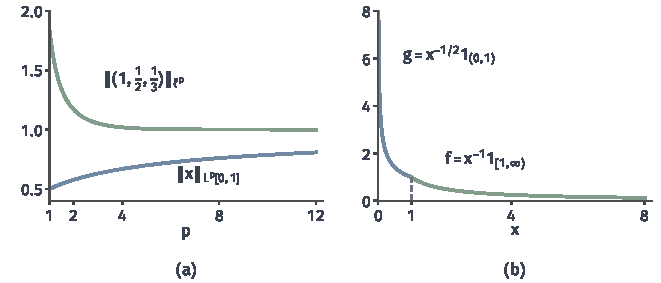
\includegraphics[width=112mm]{figures/04-spaces-measures-and-geometry/03-function-spaces/matplotlib/lop-lp-inclusion/figure.pdf}
  \caption{$L^p$范数随指数变化的方向由测度决定。(a)概率测度上$\lVert x\rVert_{L^p[0,1]}=(p+1)^{-1/p}$随$p$增大（蓝），计数测度上$(1,1/2,1/3)$的$\ell^p$范数随$p$减小（绿）。(b)$(0,\infty)$上两种失败：尖峰$g=x^{-1/2}\mathbf 1_{(0,1)}$在$L^1\setminus L^2$中（蓝），长尾$f=x^{-1}\mathbf 1_{[1,\infty)}$在$L^2\setminus L^1$中（绿）。}
  \label{fig:lop-lp-inclusion}
\end{BookInlineFigure}

\subsection{改变测度后的范数比较}
\label{sec:lop-change-of-measure}

在同一个可测空间上换一个测度，函数的$L^p$范数就要用新测度计算。设$h\geq0$可测，$\nu$由$\mathrm d\nu=h\,\mathrm d\mu$给出，即$\nu(E)=\int_Eh\,\mathrm d\mu$；第~\ref{chap:measure-densities}章把$h$称为$\nu$关于$\mu$的密度。

按向量的类比，这相当于给每个分量换一个权重$h(x)$。我们想知道$L^p(\mu)$中的误差能否控制$L^p(\nu)$中的误差，下面设$1\leq p<\infty$。

\paragraph{等价类的对应}
比较之前先要说明映射本身有意义。$L^p(\mu)$的元素是$\mu$几乎处处相等的等价类，$L^p(\nu)$的元素是$\nu$几乎处处相等的等价类。

若$f=g$在$\mu$几乎处处成立，记$N=\{f\neq g\}$，则$\mu(N)=0$，从而
\[
 \nu(N)=\int_Nh\,\mathrm d\mu=0.
\]
所以$\mu$等价类中的函数在$\nu$下也属于同一个等价类，映射$J[f]_\mu=[f]_\nu$不依赖代表的选取。这一步用的正是$\nu$关于$\mu$绝对连续：$\mu$零测集也是$\nu$零测集。

\begin{theorem}[有界密度给出有界映射]
\label{thm:lop-change-of-measure}
设$\mathrm d\nu=h\,\mathrm d\mu$，且存在常数$C$使$h\leq C$在$\mu$几乎处处成立。则对$f\in L^p(\mu)$有$f\in L^p(\nu)$，并且
\begin{equation}
 \lVert f\rVert_{L^p(\nu)}\leq C^{1/p}\lVert f\rVert_{L^p(\mu)} .
 \label{eq:lop-change-of-measure}
\end{equation}
所以$J:L^p(\mu)\to L^p(\nu)$是有界线性映射，$\lVert J\rVert\leq C^{1/p}$。
\end{theorem}

\begin{proof}
对非负可测函数$\lvert f\rvert^p$，由密度的定义，
\[
 \int\lvert f\rvert^p\,\mathrm d\nu=\int\lvert f\rvert^ph\,\mathrm d\mu\leq C\int\lvert f\rvert^p\,\mathrm d\mu.
\]
开$p$次方即得。线性由$J$在代表上作恒等变换得到。
\end{proof}

\paragraph{映射可能不是单射}
权重为零的分量不再被计入，所以$J$不一定区分$L^p(\mu)$中不同的元素。若$h=0$在某个满足$0<\mu(A)<\infty$的集合$A$上成立，则$\mathbf 1_A$在$L^p(\mu)$中非零，但
\[
 \int\mathbf 1_A\,\mathrm d\nu=\int_Ah\,\mathrm d\mu=0,
\]
所以$J\mathbf 1_A=0$。新测度看不见$A$上发生的事情，$\ker J$由在$\{h>0\}$上几乎处处为零的函数组成。

若$h>0$在$\mu$几乎处处成立，两种零测集就一致。一方面，绝对连续已给出由$\mu(E)=0$推出$\nu(E)=0$。另一方面，若$\nu(E)=\int_Eh\,\mathrm d\mu=0$，则$h\mathbf 1_E=0$在$\mu$几乎处处成立，而$h>0$几乎处处，只能$\mathbf 1_E=0$几乎处处，即$\mu(E)=0$。

这时两种等价类相同，$J$是单射；但$h$可以任意接近零，$J$仍可能不满射，逆映射也可能无界。在$[0,1]$上取$h(x)=x$，函数$x^{-3/4}$满足$\int x^{-3/2}\cdot x\,\mathrm dx<\infty$，属于$L^2(\nu)$，而$\int x^{-3/2}\,\mathrm dx=\infty$，不属于$L^2(\mu)$，所以$J$不是满射。

若密度还有正下界，即$0<c\leq h\leq C$几乎处处，同样的计算给出
\begin{equation}
 c^{1/p}\lVert f\rVert_{L^p(\mu)}\leq\lVert f\rVert_{L^p(\nu)}\leq C^{1/p}\lVert f\rVert_{L^p(\mu)} .
 \label{eq:lop-measure-equivalence}
\end{equation}
这时$L^p(\mu)$与$L^p(\nu)$是同一个函数空间，两个范数等价。例如在$[0,1]$上取$h(x)=1+x$，有$1\leq h\leq2$，两个$L^2$范数之比始终在$1$与$\sqrt2$之间。

若取$h(x)=x$，下界消失。令$f_n=\sqrt n\,\mathbf 1_{(0,1/n)}$，则$\lVert f_n\rVert_{L^2(\mu)}=1$，而
\[
 \lVert f_n\rVert_{L^2(\nu)}^2=n\int_0^{1/n}x\,\mathrm dx=\frac1{2n}\to0.
\]
反方向的控制不存在。权重越接近零的区域，越能藏住$\mu$意义下的大函数。

\section{算子列的收敛}
\label{sec:lop-operator-convergence}

实际计算中，我们常用一列逐渐精细的近似算子$T_n$代替一个算子$T$，例如只保留前$n$个展开系数，或者把积分区域截去一小块。对手中的每个输入，近似输出会越来越准；但这是否意味着存在一个只依赖$n$的误差界，对所有单位输入同时有效？

有限维中这不成问题：矩阵的每个元素收敛，整个矩阵就按任何范数收敛。无限维中矩阵有无穷多列，“每一列都收敛”和“所有列一起收敛”不再是一回事，这两种要求的量词次序不同，强弱也不同。

\begin{definition}[算子范数收敛与强算子收敛]
\label{def:lop-operator-convergence}
设$X,Y$是赋范空间，$T_n,T\in\mathcal B(X,Y)$。若
\begin{equation}
 \lVert T_n-T\rVert\to0,
 \label{eq:lop-norm-convergence}
\end{equation}
则称$T_n$\term{算子范数收敛}（convergence in operator norm）到$T$。若
\begin{equation}
 \lVert T_nx-Tx\rVert_Y\to0\qquad(\text{对每个}x\in X),
 \label{eq:lop-strong-convergence}
\end{equation}
则称$T_n$\term{强算子收敛}（strong operator convergence）到$T$。
\end{definition}

算子范数收敛给出统一误差：$\lVert T_n-T\rVert$只依赖$n$，对单位球中的全部输入同时控制输出误差。强算子收敛给出逐输入误差：先固定$x$，再让$n\to\infty$，收敛快慢可以随$x$变化。由
\[
 \lVert T_nx-Tx\rVert\leq\lVert T_n-T\rVert\,\lVert x\rVert,
\]
算子范数收敛蕴含强算子收敛；下面的例子说明反过来不成立。

强算子收敛中的“逐点”，指的是对每个输入向量$x$，像向量$T_nx$在$Y$的范数下收敛。当$X,Y$是函数空间时，它不是说函数$T_nx$在定义域的每个点处收敛，后者是函数列的另一种收敛方式，二者不能混用。

\paragraph{截断投影}
设$H$是无限维可分Hilbert空间，$(e_k)_{k\geq1}$是标准正交基，$P_n$是到$\operatorname{span}\{e_1,\ldots,e_n\}$的正交投影，即
\[
 P_nx=\sum_{k\leq n}\langle e_k,x\rangle e_k.
\]
按第~\ref{sec:lop-norm-definition}小节的矩阵表示，$P_n$是对角矩阵$\operatorname{diag}(1,\ldots,1,0,0,\ldots)$，前$n$个对角元素为$1$。

固定$x$。由第~\ref{chap:function-inner-product-spaces}章的Parseval等式，
\[
 \lVert x-P_nx\rVert^2=\sum_{k>n}\lvert\langle e_k,x\rangle\rvert^2\to0,
\]
因为右端是一个收敛级数的尾部，这个级数的和是$\lVert x\rVert^2$。所以$P_n$强算子收敛到恒等算子$I$。

另一方面，对每个$n$，被截掉的单位向量$e_{n+1}$满足$P_ne_{n+1}=0$，于是
\[
 \lVert(I-P_n)e_{n+1}\rVert=1.
\]
又$I-P_n$是到正交补的投影，$\lVert I-P_n\rVert\leq1$。所以$\lVert I-P_n\rVert=1$对一切$n$成立，$P_n$不按算子范数收敛到$I$。在矩阵上看，差$I-P_n$是$\operatorname{diag}(0,\ldots,0,1,1,\ldots)$，对角线上总还有$1$。

图~\ref{fig:lop-projection-strong-norm}比较了三个输入的截断误差。系数为$2^{-k/2}$的单位向量，其截断误差为$2^{-n/2}$，衰减很快；系数与$1/k$成比例的单位向量衰减慢得多。

\begin{BookInlineFigure}
  \centering
  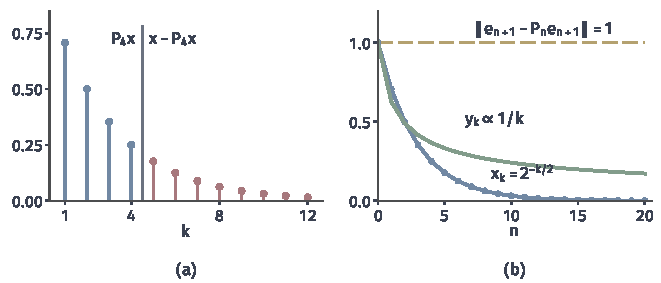
\includegraphics[width=112mm]{figures/04-spaces-measures-and-geometry/03-function-spaces/matplotlib/lop-projection-strong-norm/figure.pdf}
  \caption{截断投影的强收敛与算子范数不收敛。(a)单位向量$x$的系数$c_k=2^{-k/2}$，$P_4$保留蓝色的前四项，红色尾项构成误差$x-P_4x$。(b)截断误差随保留项数$n$的变化：$\lVert x-P_nx\rVert=2^{-n/2}$（蓝），系数与$1/k$成比例的单位向量$y$（绿）衰减较慢，而被截掉的基向量$e_{n+1}$的误差始终为$1$（黄虚线）。}
  \label{fig:lop-projection-strong-norm}
\end{BookInlineFigure}

每个固定输入的误差都趋于零，但不同输入的速度可以任意慢，而被截掉的那个基向量的误差始终是$1$。“每个元素都能被有限维子空间逼近”并不意味着同一个有限维子空间能以任意精度统一逼近整个单位球。

\paragraph{有限个输入上的统一控制}
强算子收敛对有限个输入仍可同时控制。设$x^{(1)},\ldots,x^{(m)}$是固定的输入，对每个$i$取$N_i$使误差小于$\varepsilon$，再取$N=\max_iN_i$即可。

截断投影失去统一控制的原因是单位球中有无穷多个相互正交的方向，每个$P_n$只能照顾其中有限个。第~\ref{sec:lop-uniform-boundedness}小节将说明，在Banach空间上，强算子收敛的算子列至少有统一的范数上界。

\paragraph{函数空间中的截断}
在$L^2(0,1)$中，按二分区间依次排列
\[
 I_1=[0,1],\quad I_2=[0,\tfrac12],\quad I_3=[\tfrac12,1],\quad I_4=[0,\tfrac14],\ \ldots,
\]
长度$\lvert I_n\rvert\to0$。令$T_nf=(1-\mathbf 1_{I_n})f$，即把输入在$I_n$上的部分抹去，这是一个乘法算子。对每个$f\in L^2$，
\[
 \lVert f-T_nf\rVert_2^2=\int_{I_n}\lvert f\rvert^2\,\mathrm dx\to0,
\]
因为$\lvert f\rvert^2$可积，积分区域的测度趋于零时积分趋于零。所以$T_n$强算子收敛到$I$。

同一列算子却不按算子范数收敛。取$f_n=\lvert I_n\rvert^{-1/2}\mathbf 1_{I_n}$，它是单位向量且$(I-T_n)f_n=f_n$，故$\lVert I-T_n\rVert=1$。

更值得注意的是，取$f=1$，每个$x\in[0,1]$都落在无穷多个$I_n$中，也落在无穷多个$I_n$之外。于是$(T_nf)(x)$在$0$与$1$之间无穷次跳动，对任何$x$都不收敛。强算子收敛成立，输出函数却在每一点都不收敛，这正说明二者是不同的概念。

\section{伴随算子}
\label{sec:lop-adjoint}

矩阵有共轭转置，它在算子上的对应物叫做伴随。定义的动机来自观测：算子$T:H_1\to H_2$把输入送进输出空间，我们却常常只能用一个测试方向去观察输出，例如读出$Tx$在某个单位向量$v$上的分量$\langle v,Tx\rangle$。

这个读数对$x$是线性的，因而是输入空间上的一个泛函。第~\ref{chap:linear-functionals}章说明，Hilbert空间上的连续线性泛函都可以写成内积；于是每个输出方向$v$都对应输入空间中的一个方向。本节用这一对应定义伴随，并研究输入中哪些方向在输出中看不见、输出中哪些方向够不着。

本节设$H_1,H_2,H_3$是同一标量域上的Hilbert空间，算子都定义在整个输入空间上并且有界。复内积沿用第~\ref{chap:function-inner-product-spaces}章的约定：对第一个变量共轭线性，对第二个变量线性。

\subsection{伴随的定义}
\label{sec:lop-adjoint-def}

固定$T\in\mathcal B(H_1,H_2)$与输出方向$v\in H_2$，考察读数$x\mapsto\langle v,Tx\rangle$。它对$x$线性，并且
\[
 \lvert\langle v,Tx\rangle\rvert\leq\lVert v\rVert\,\lVert T\rVert\,\lVert x\rVert,
\]
所以是$H_1$上的有界线性泛函。由Riesz表示定理，存在唯一的$w\in H_1$，使$\langle v,Tx\rangle=\langle w,x\rangle$对一切$x\in H_1$成立。这个$w$随$v$而定。

\begin{definition}[伴随算子]
\label{def:lop-adjoint}
设$T\in\mathcal B(H_1,H_2)$。对每个$v\in H_2$，令$T^*v\in H_1$为满足
\begin{equation}
 \langle v,Tx\rangle_{H_2}=\langle T^*v,x\rangle_{H_1}\qquad(x\in H_1)
 \label{eq:lop-adjoint}
\end{equation}
的唯一元素。映射$T^*:H_2\to H_1$称为$T$的\term{伴随}（adjoint）算子。
\end{definition}

伴随把测试方向从输出空间拉回输入空间：用$v$测试$Tx$，相当于用$T^*v$测试$x$。它的定义域是整个输出空间$H_2$，取值空间是输入空间$H_1$，方向与$T$相反；它不是从输出恢复输入，后面的移位算子会说明这一区别。

\begin{theorem}[伴随的基本性质]
\label{thm:lop-adjoint-properties}
设$S,T\in\mathcal B(H_1,H_2)$，$R\in\mathcal B(H_2,H_3)$，$\alpha\in\mathbb F$。则$T^*\in\mathcal B(H_2,H_1)$，并且
\begin{equation}
 \begin{gathered}
 (S+T)^*=S^*+T^*,\quad(\alpha T)^*=\bar\alpha T^*,\quad(RT)^*=T^*R^*,\\
 T^{**}=T,\quad\lVert T^*\rVert=\lVert T\rVert,\quad\lVert T^*T\rVert=\lVert T\rVert^2 .
 \end{gathered}
 \label{eq:lop-adjoint-properties}
\end{equation}
\end{theorem}

\begin{proof}
先证线性。对$v_1,v_2\in H_2$及标量$\beta_1,\beta_2$，由内积对第一个变量共轭线性，
\[
 \begin{aligned}
 \langle T^*(\beta_1v_1+\beta_2v_2),x\rangle
 &=\langle\beta_1v_1+\beta_2v_2,Tx\rangle\\
 &=\bar\beta_1\langle T^*v_1,x\rangle+\bar\beta_2\langle T^*v_2,x\rangle\\
 &=\langle\beta_1T^*v_1+\beta_2T^*v_2,x\rangle ,
 \end{aligned}
\]
对一切$x$成立，由表示的唯一性得线性。

和、数乘与复合的公式用同样的方式验证。复合的情形是
\[
 \langle v,RTx\rangle=\langle R^*v,Tx\rangle=\langle T^*R^*v,x\rangle.
\]
数乘公式中出现$\bar\alpha$，是因为把标量移进第一个变量要取共轭：
\[
 \langle v,\alpha Tx\rangle=\alpha\langle T^*v,x\rangle=\langle\bar\alpha T^*v,x\rangle.
\]

再证有界与范数。由式~\eqref{eq:lop-adjoint}，
\[
 \lVert T^*v\rVert^2=\langle T^*v,T^*v\rangle=\langle v,TT^*v\rangle\leq\lVert v\rVert\,\lVert T\rVert\,\lVert T^*v\rVert,
\]
两边约去$\lVert T^*v\rVert$（它为零时不等式自然成立），即得$\lVert T^*\rVert\leq\lVert T\rVert$。

对式~\eqref{eq:lop-adjoint}两边取共轭得$\langle x,T^*v\rangle=\langle Tx,v\rangle$，这说明$T$满足$T^*$的伴随所需的等式，故$T^{**}=T$。把刚才的不等式用于$T^*$，就得到反方向的$\lVert T\rVert\leq\lVert T^*\rVert$。

最后，由复合的范数估计，
\[
 \lVert T^*T\rVert\leq\lVert T^*\rVert\,\lVert T\rVert=\lVert T\rVert^2.
\]
另一方面对单位向量$x$，
\[
 \lVert Tx\rVert^2=\langle x,T^*Tx\rangle\leq\lVert T^*T\rVert,
\]
取上确界得$\lVert T\rVert^2\leq\lVert T^*T\rVert$。
\end{proof}

在$\mathbb C^n$与$\mathbb C^m$上配标准内积$\langle\bm v,\bm w\rangle=\bm v^*\bm w$，矩阵$\bm A$满足
\[
 \langle\bm v,\bm A\bm x\rangle=\bm v^*\bm A\bm x=(\bm A^*\bm v)^*\bm x,
\]
所以它的伴随是共轭转置$\bm A^*$；实情形就是转置。共轭来自内积约定本身，不能把伴随只当作“转置”的记号：在复空间中直接用转置，等式~\eqref{eq:lop-adjoint}一般不成立。式~\eqref{eq:lop-matrix-entry}的矩阵元素同样满足$(T^*)_{mn}=\overline{A_{nm}}$。

\paragraph{累积积分的伴随}
在$L^2(0,1)$上令$(Vf)(s)=\int_0^sf(t)\,\mathrm dt$，即从$0$累积到$s$。它是核为$\mathbf 1_{\{t<s\}}$的积分算子，核在$[0,1]^2$上平方可积，由定理~\ref{thm:lop-hs-bounded}有界。按矩阵看，第$s$行在列$t<s$处都是$1$，这是一个下三角矩阵。

转置以后应当是上三角矩阵。对$g\in L^2(0,1)$，被积函数$\overline{g(s)}f(t)\mathbf 1_{\{t<s\}}$在单位正方形上可积，由Fubini定理交换积分次序，
\[
 \begin{aligned}
 \langle g,Vf\rangle
 &=\int_0^1\overline{g(s)}\int_0^sf(t)\,\mathrm dt\,\mathrm ds\\
 &=\int_0^1\overline{\Bigl(\int_t^1g(s)\,\mathrm ds\Bigr)}f(t)\,\mathrm dt ,
 \end{aligned}
\]
所以$(V^*g)(t)=\int_t^1g(s)\,\mathrm ds$，即从$t$累积到$1$。

用$f=g=1$核对。左边是
\[
 \langle1,V1\rangle=\int_0^1s\,\mathrm ds=\frac12.
\]
又$V^*1=1-t$，右边是
\[
 \langle V^*1,1\rangle=\int_0^1(1-t)\,\mathrm dt=\frac12,
\]
两边相等。

\paragraph{伴随不是逆}
在$\ell^2$上，右移$S$的伴随是左移
\[
 S^*(y_1,y_2,\ldots)=(y_2,y_3,\ldots),
\]
逐项核对即得
\[
 \langle y,Sx\rangle=\sum_{k\geq1}\bar y_{k+1}x_k=\langle S^*y,x\rangle.
\]
矩阵上，$S$的$1$在主对角线下方一条斜线，转置后移到上方一条斜线。

于是$S^*S=I$，左移撤销了右移。但$SS^*(y_1,y_2,\ldots)=(0,y_2,y_3,\ldots)$抹掉了第一个坐标，$SS^*\neq I$。$S$保持长度，不丢失信息，只是它的像缺少$e_1$方向，所以$S^*$只是左逆。

这个例子同时说明无限维中单射不等于满射：$S$是单射而非满射，$S^*$是满射而非单射。对一般算子，伴随连左逆都不是：零算子的伴随仍是零算子。

\subsection{像与零空间的正交关系}
\label{sec:lop-range-kernel}

伴随的定义式把“输出方向$v$与一切$Tx$正交”翻译成输入空间中的条件$\langle T^*v,x\rangle=0$对一切$x$成立，也就是$T^*v=0$。由此得到像与零空间之间的正交关系。

\begin{theorem}[像与零空间的正交关系]
\label{thm:lop-range-kernel}
设$T\in\mathcal B(H_1,H_2)$。则
\begin{equation}
 (\operatorname{Ran}T)^\perp=\ker T^*,\qquad\overline{\operatorname{Ran}T}=(\ker T^*)^\perp ,
 \label{eq:lop-range-kernel}
\end{equation}
交换$T$与$T^*$的角色，又有$(\operatorname{Ran}T^*)^\perp=\ker T$与$\overline{\operatorname{Ran}T^*}=(\ker T)^\perp$。
\end{theorem}

\begin{proof}
$v\in(\operatorname{Ran}T)^\perp$当且仅当对一切$x$有$\langle v,Tx\rangle=0$，即$\langle T^*v,x\rangle=0$对一切$x$成立。取$x=T^*v$可知这等价于$T^*v=0$。这证明了第一个等式。

对第二个等式，只需说明线性子空间$M$满足$(M^\perp)^\perp=\overline M$，再取$M=\operatorname{Ran}T$。由定义$M\subseteq(M^\perp)^\perp$，后者是闭集，所以$\overline M\subseteq(M^\perp)^\perp$。

反过来，设$v\in(M^\perp)^\perp$，作正交分解$v=P_{\overline M}v+z$，其中$z\perp\overline M$，从而$z\in M^\perp$。$v$与$P_{\overline M}v$都与$z$正交，所以
\[
 \lVert z\rVert^2=\langle z,v-P_{\overline M}v\rangle=0,
\]
即$v\in\overline M$。其余两式把$T$换成$T^*$并用$T^{**}=T$即得。
\end{proof}

由此得到两个空间的正交分解
\begin{equation}
 H_1=\ker T\oplus\overline{\operatorname{Ran}T^*},\qquad H_2=\ker T^*\oplus\overline{\operatorname{Ran}T}.
 \label{eq:lop-four-subspaces}
\end{equation}
$\ker T$中的输入方向在输出中完全看不见，加到任何输入上都不改变输出。$\overline{\operatorname{Ran}T}$是能被输出逼近的方向。$\ker T^*$中的输出方向与一切输出正交，任何输入都到达不了。

图~\ref{fig:lop-four-subspaces}把四个子空间放在一起。这是矩阵的“四个基本子空间”在Hilbert空间中的形式，区别在于像必须取闭包。

\begin{BookInlineFigure}
  \centering
  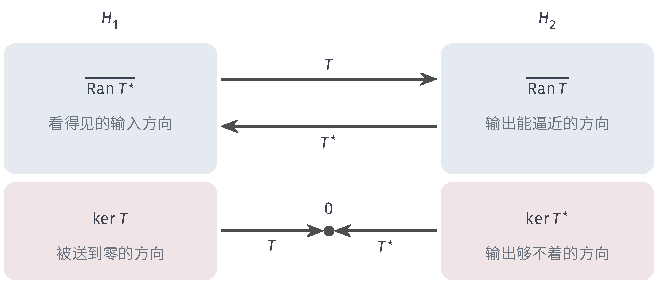
\includegraphics[width=111.404mm]{figures/04-spaces-measures-and-geometry/03-function-spaces/tikz/lop-four-subspaces/figure.pdf}
  \caption{伴随与像、零空间的正交关系。输入空间$H_1$分解为$\overline{\operatorname{Ran}T^*}$与$\ker T$，输出空间$H_2$分解为$\overline{\operatorname{Ran}T}$与$\ker T^*$。$T$把$\ker T$送到零，其余方向的像落在$\operatorname{Ran}T$中；$T^*$把$\ker T^*$送到零。无限维中像未必闭，正交关系只确定像的闭包。}
  \label{fig:lop-four-subspaces}
\end{BookInlineFigure}

\paragraph{像稠密而不闭}
闭包在无限维中不能省去。回到$\ell^2$上的对角算子$A(x_n)=(x_n/n)$。逐项核对可知$A^*=A$，且$A$是单射，所以$\ker A^*=\{0\}$，由式~\eqref{eq:lop-range-kernel}，$\operatorname{Ran}A$在$\ell^2$中稠密。

考察$y=(1/n)$，它满足$\sum_n1/n^2<\infty$，属于$\ell^2$。若$Ax=y$，逐个坐标比较得$x_n=1$，这个唯一的候选不是平方可和的，所以$y\notin\operatorname{Ran}A$。

截断候选可以看清发生了什么。令$x^{(N)}$为前$N$个坐标为$1$、其余为$0$的序列，则
\[
 \lVert Ax^{(N)}-y\rVert^2=\sum_{n>N}\frac{1}{n^2}\to0,\qquad\lVert x^{(N)}\rVert=\sqrt N\to\infty .
\]
残差趋于零，说明$y$在像的闭包中；为了取得这些越来越好的近似，输入的范数却无限增大。$y$是“只能逼近”的输出，而不是“真正属于像”的输出。

累积积分$V$给出同样的现象。若$V^*g=0$，则$\int_t^1g=0$对一切$t$成立，于是$g$在每个区间上积分为零，即$g$与一切区间示性函数正交。区间示性函数的线性组合在$L^2(0,1)$中稠密（第~\ref{chap:wavelet-transform}章用二分阶梯函数证明了这一点），所以$g=0$几乎处处，$\ker V^*=\{0\}$，$\operatorname{Ran}V$稠密。

但$\operatorname{Ran}V$中的函数都连续，阶跃函数$\mathbf 1_{(1/2,1)}$不在其中，所以$\operatorname{Ran}V\neq L^2(0,1)$。

因此，$v\perp\ker T^*$只能保证$v$在像的闭包中，不能保证方程$Tx=v$精确可解。只有已知$\operatorname{Ran}T$闭时，才有$\operatorname{Ran}T=(\ker T^*)^\perp$，这时可解性等价于与$\ker T^*$正交。何时像闭、近似解的输入为何会爆炸，是第~\ref{chap:linear-operator-equations}章的问题。

\subsection{自伴算子}
\label{sec:lop-self-adjoint}

当输入与输出在同一个Hilbert空间$H$中时，$T$与$T^*$都属于$\mathcal B(H)$，可以直接比较。实对称矩阵与复Hermite矩阵的伴随就是它自己，下面把这一性质推广到一般Hilbert空间。

\begin{definition}[自伴算子]
\label{def:lop-self-adjoint}
设$T\in\mathcal B(H)$。若$T^*=T$，即
\begin{equation}
 \langle v,Tx\rangle=\langle Tv,x\rangle\qquad(x,v\in H),
 \label{eq:lop-self-adjoint}
\end{equation}
则称$T$为\term{自伴}（self-adjoint）算子。
\end{definition}

自伴算子的二次型$\langle x,Tx\rangle$总是实数，因为
\[
 \langle x,Tx\rangle=\langle Tx,x\rangle=\overline{\langle x,Tx\rangle}.
\]
累积积分$V$不自伴，因为$V^*$从$t$累积到$1$而$V$从$0$累积到$t$；右移$S$也不自伴。

\paragraph{正交投影}
设$M$是闭子空间，$P=P_M$。对任意$x,z\in H$，$z-Pz\perp M$而$Px\in M$，所以
\[
 \langle z,Px\rangle=\langle Pz,Px\rangle+\langle z-Pz,Px\rangle=\langle Pz,Px\rangle.
\]
同理$\langle Pz,x\rangle=\langle Pz,Px\rangle$。两式相比得$\langle z,Px\rangle=\langle Pz,x\rangle$，即$P^*=P$。正交投影是自伴的；只满足$P^2=P$而像与零空间不正交的斜投影则不是。

\paragraph{积分算子的伴随核}
矩阵的共轭转置，是把元素$K_{ij}$放到$(j,i)$位置并取共轭。积分算子的伴随也是这样，核由交换变量并取共轭得到。设$(X,\mu)$、$(Y,\nu)$是$\sigma$有限测度空间，$k\in L^2(X\times Y,\mu\otimes\nu)$，$T:L^2(Y,\nu)\to L^2(X,\mu)$由式~\eqref{eq:lop-integral-operator}给出。

\begin{theorem}[伴随核]
\label{thm:lop-adjoint-kernel}
在上述条件下，$T^*:L^2(X,\mu)\to L^2(Y,\nu)$是以$k^*(y,x)=\overline{k(x,y)}$为核的积分算子，即
\begin{equation}
 (T^*g)(y)=\int_X\overline{k(x,y)}g(x)\,\mathrm d\mu(x).
 \label{eq:lop-adjoint-kernel}
\end{equation}
\end{theorem}

\begin{proof}
任取$f\in L^2(\nu)$、$g\in L^2(\mu)$。函数$(x,y)\mapsto\lvert g(x)\rvert\,\lvert k(x,y)\rvert\,\lvert f(y)\rvert$在乘积空间上可积：由乘积空间中的Cauchy--Schwarz不等式，它的积分不超过$\lVert k\rVert_{L^2}$乘以$(x,y)\mapsto\lvert g(x)f(y)\rvert$的$L^2$范数，后者由Tonelli定理等于$\lVert g\rVert\,\lVert f\rVert$。

于是可以用Fubini定理交换积分次序：
\[
 \begin{aligned}
 \langle g,Tf\rangle&=\int_X\overline{g(x)}\int_Yk(x,y)f(y)\,\mathrm d\nu(y)\,\mathrm d\mu(x)\\
 &=\int_Y\overline{\Bigl(\int_X\overline{k(x,y)}g(x)\,\mathrm d\mu(x)\Bigr)}f(y)\,\mathrm d\nu(y).
 \end{aligned}
\]
$k^*$在$Y\times X$上平方可积，由定理~\ref{thm:lop-hs-bounded}，括号中的函数属于$L^2(\nu)$。上式说明它满足伴随的定义式，由唯一性，它就是$T^*g$。
\end{proof}

当$X=Y$且$\mu=\nu$时，若$k(x,y)=\overline{k(y,x)}$对$\mu\otimes\mu$几乎处处的$(x,y)$成立，则$k^*=k$几乎处处，由定理得$T^*=T$，积分算子自伴。实值核的这一条件就是对称性$k(x,y)=k(y,x)$，相当于矩阵的对称。条件只需几乎处处成立：在零测集上改动核不改变积分算子。

贯穿例子的$1+xz$是实对称核，所以式~\eqref{eq:lop-running-kernel}给出自伴算子。累积积分的核$\mathbf 1_{\{t<s\}}$关于对角线不对称，伴随核是它的镜像，图~\ref{fig:lop-kernel-adjoint}用方格画出了这个下三角矩阵及其转置。

\begin{BookInlineFigure}
  \centering
  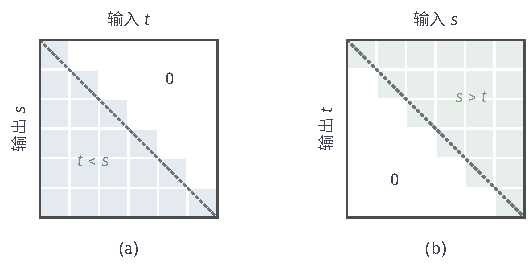
\includegraphics[width=89.623mm]{figures/04-spaces-measures-and-geometry/03-function-spaces/tikz/lop-kernel-adjoint/figure.pdf}
  \caption{积分核与伴随核关于对角线互为镜像，方格表示把区间六等分后的矩阵，虚线是连续极限下的边界，列从左到右、行从上到下对应变量增大。(a)$V$的核$\mathbf 1_{\{t<s\}}$，填色处取值$1$，是下三角矩阵。(b)伴随$V^*$的核$\mathbf 1_{\{s>t\}}$，是上三角矩阵。两核不相等，所以$V$不自伴。}
  \label{fig:lop-kernel-adjoint}
\end{BookInlineFigure}

\subsection{正算子}
\label{sec:lop-positive}

自伴保证二次型$\langle x,Tx\rangle$是实数，但这个实数可正可负。很多场合需要它非负：例如$\langle x,T^*Tx\rangle=\lVert Tx\rVert^2$度量输出的能量。这相当于矩阵的半正定，给出比自伴更强的条件。

\begin{definition}[正算子]
\label{def:lop-positive-operator}
设$T\in\mathcal B(H)$自伴。若
\begin{equation}
 \langle x,Tx\rangle\geq0\qquad(x\in H),
 \label{eq:lop-positive}
\end{equation}
则称$T$为\term{正算子}（positive operator），记作$T\geq0$。
\end{definition}

两个基本例子是正交投影与$T^*T$。对正交投影，
\[
 \langle x,Px\rangle=\langle Px,Px\rangle=\lVert Px\rVert^2\geq0.
\]
对任意$T\in\mathcal B(H_1,H_2)$，$T^*T\in\mathcal B(H_1)$自伴，因为$(T^*T)^*=T^*T^{**}=T^*T$，并且
\[
 \langle x,T^*Tx\rangle=\langle Tx,Tx\rangle=\lVert Tx\rVert^2\geq0.
\]

\paragraph{自伴条件与二次型非负条件}
定义把两个条件分开写出，因为在实空间中二次型非负并不能推出自伴。平面上逆时针旋转$90^\circ$的矩阵
\[
 \bm R=\begin{bmatrix}0&-1\\1&0\end{bmatrix}
\]
满足$\bm x^{\top}\bm R\bm x=-x_1x_2+x_2x_1=0$，二次型非负，却不对称。

复Hilbert空间中情况不同：二次型对一切$x$取实值已经迫使算子自伴。记$B=T-T^*$，它的二次型为
\[
 \langle x,Bx\rangle=\langle x,Tx\rangle-\langle Tx,x\rangle=2\mathrm i\operatorname{Im}\langle x,Tx\rangle=0.
\]

把$x+v$代入$\langle x,Bx\rangle=0$并展开，得到
\[
 \langle x,Bv\rangle+\langle v,Bx\rangle=0.
\]
再把$v$换成$\mathrm iv$，由第一个变量的共轭线性，得到
\[
 \mathrm i\langle x,Bv\rangle-\mathrm i\langle v,Bx\rangle=0.
\]
两式合起来给出$\langle x,Bv\rangle=0$对一切$x,v$成立，所以$B=0$。

为了使定义在实、复两种情形下一致，我们仍把自伴列为前提。反过来，自伴也不推出二次型非负，下面的积分算子就是例子。

\paragraph{积分算子的正性}
对$L^2(\mu)$上满足$k(x,y)=\overline{k(y,x)}$的平方可积核，自伴积分算子的正性由积分二次型检验：
\begin{equation}
 \langle f,Tf\rangle=\iint\overline{f(x)}\,k(x,y)\,f(y)\,\mathrm d\mu(y)\,\mathrm d\mu(x)\geq0\qquad(f\in L^2(\mu)).
 \label{eq:lop-integral-positive}
\end{equation}
这是矩阵半正定条件$\bm f^*\bm K\bm f\geq0$的连续版本。

贯穿例子中，
\[
 \langle f,Tf\rangle=\Bigl\lvert\int f\,\mathrm d\mu\Bigr\rvert^2+\Bigl\lvert\int zf\,\mathrm d\mu\Bigr\rvert^2\geq0,
\]
所以它是正算子。把核换成$1-6xz$，算子仍自伴，但取$f=x$，由$\int z\,\mathrm d\mu=0$与$\int z^2\,\mathrm d\mu=1/3$得
\[
 Tf=-2x,\qquad\langle f,Tf\rangle=-2\int x^2\,\mathrm d\mu=-\frac23<0,
\]
它不是正算子。

\paragraph{核逐点非负不等于正算子}
矩阵元素全为正的矩阵未必半正定，核也是如此。取两点集合$\{1,2\}$配计数测度，此时$L^2$就是$\mathbb F^2$，积分就是求和。核$k(1,1)=k(2,2)=0$、$k(1,2)=k(2,1)=1$逐点非负且对称，对应的算子交换两个坐标，矩阵为$\left[\begin{smallmatrix}0&1\\1&0\end{smallmatrix}\right]$。

取$f=(1,-1)$，$Tf=(-1,1)$，于是$\langle f,Tf\rangle=-2<0$。

反方向也不成立：核$k(x,z)=xz$在$x=1,z=-1$处为负，却给出
\[
 \langle f,Tf\rangle=\Bigl\lvert\int zf\,\mathrm d\mu\Bigr\rvert^2\geq0
\]
的正算子。正性是关于所有输入的二次型的条件，不能由核在单个点上的符号判断。

\section{紧算子}
\label{sec:lop-compact}

有界算子把有界输入变成有界输出，但无限维空间中有界序列未必有收敛子列，所以有界性本身不保证输出能被有限多个代表近似。本节要求有界输入列的输出能选出范数收敛的子列，由此得到比有界性更强的紧性。我们先比较有限秩算子与无限维恒等算子，再在Hilbert空间中建立有限秩逼近，最后把结论用于平方可积核的积分算子。

\subsection{紧算子的定义}
\label{sec:lop-compact-def}

第~\ref{chap:topological-spaces}章把闭包紧的集合称为相对紧集；第~\ref{chap:metric-spaces}章说明，在度量空间中，集合相对紧当且仅当其中每个序列都有在全空间中收敛的子列，并且在完备度量空间中这又等价于全有界，即对每个$\varepsilon>0$都能被有限个半径$\varepsilon$的球覆盖。下面把这一性质加在算子的像上。

先看输出落在有限维空间中的情形。有界线性算子$F:X\to Y$若像$\operatorname{Ran}F$是有限维子空间，就称为\term{有限秩算子}（finite-rank operator），$\dim\operatorname{Ran}F$称为它的秩。若$\lVert x_n\rVert\leq C$，则$\lVert Fx_n\rVert\leq\lVert F\rVert C$，输出序列落在有限维空间的一个有界集合中。有限维赋范空间中所有范数等价，有界序列总有收敛子列，所以$(Fx_n)$有范数收敛的子列。

\begin{definition}[紧算子]
\label{def:lop-compact-operator}
设$X,Y$是赋范空间，$T:X\to Y$是线性算子。若$X$的闭单位球$B_X$的像$T(B_X)$在$Y$中相对紧，则称$T$为\term{紧算子}（compact operator）。等价地，对$X$中每个有界序列$(x_n)$，输出序列$(Tx_n)$都有在$Y$中按范数收敛的子列。
\end{definition}

两种说法等价，是因为有界序列经缩放后落在某个$rB_X$中，而$T(rB_X)=rT(B_X)$与$T(B_X)$同时相对紧。紧算子必然有界：若$T$无界，可取单位向量$x_n$使$\lVert Tx_n\rVert\geq n$，输出序列的任何子列都无界，不可能收敛。由上一段，每个有界有限秩算子都是紧算子。

\paragraph{无限维恒等算子不紧}
紧性不是每个有界算子都具备的。设$H$是无限维Hilbert空间，取标准正交序列$(e_n)$。对$n\neq m$，$\lVert e_n-e_m\rVert^2=\lVert e_n\rVert^2+\lVert e_m\rVert^2=2$。恒等算子$I$把这个有界序列原样输出，任意两项相距$\sqrt2$，没有柯西子列，因而没有收敛子列，$I$不是紧算子。一般的无限维赋范空间中，第~\ref{chap:functions-as-vectors}章用Riesz引理说明闭单位球不紧，所以恒等算子同样不紧。

同一个序列经过$\ell^2$上的对角算子$A(x_n)=(x_n/n)$后变成$Ae_n=e_n/n$，按范数趋于零。图~\ref{fig:lop-identity-orthonormal}比较了两种输出。$A$的单位球像满足$\lvert(Ax)_n\rvert\leq1/n$，越靠后的方向被压得越扁；下一小节将用有限秩逼近证明它是紧算子。

\begin{figure}[!htb]
  \centering
  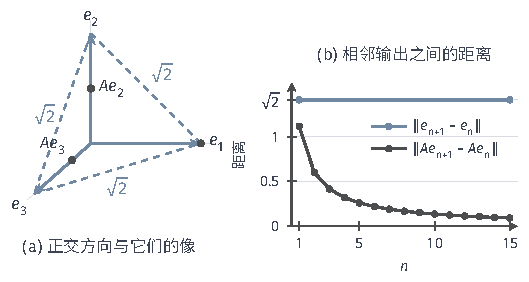
\includegraphics[width=89.6mm]{figures/02-abstract-mathematics/03-function-spaces/tikz/c3-identity-orthonormal/figure.pdf}
  \caption{同一个标准正交序列经过恒等算子与经过$A(x_n)=(x_n/n)$的对比。(a)~$e_1,e_2,e_3$两两相距$\sqrt2$（虚线），它们在$A$下的像$e_1$、$e_2/2$、$e_3/3$（黑点）向原点收拢；(b)~相邻输出的距离在恒等算子下恒为$\sqrt2$，在$A$下等于$\sqrt{1/n^2+1/(n+1)^2}$并趋于零。}
  \label{fig:lop-identity-orthonormal}
\end{figure}

这个例子说明紧性约束的对象。每个$x\in H$都能被它在前$n$个基向量上的截断任意逼近，单独看每个元素，有限截断都可行；紧性要求的却是同一个算子作用于整个有界输入族之后，输出整体可以被有限个代表覆盖。恒等算子对每个输入都能截断，对整个单位球却不能。

\paragraph{弱收敛的输入与范数收敛的输出}
第~\ref{chap:linear-functionals}章的标准正交序列满足$e_n\rightharpoonup0$而不按范数收敛。上例中$Ae_n=e_n/n$却按范数收敛到$A0=0$。这不是巧合：紧算子把弱收敛的输入变成范数收敛的输出。需要区分的是，弱收敛是输入列在全部连续线性观测下的收敛，相对紧是输出集合在范数距离下的性质，定理说明紧性在二者之间架起桥梁。

\begin{theorem}[紧算子改善收敛]
\label{thm:lop-compact-weak-strong}
设$X,Y$是赋范空间，$T:X\to Y$是紧算子。若$x_n\rightharpoonup x$，则$\lVert Tx_n-Tx\rVert\to0$。
\end{theorem}

\begin{proof}
第一步，输出弱收敛。对每个$\ell\in Y^*$，复合$\ell\circ T$是$X$上的有界线性泛函，所以$\ell(Tx_n)\to\ell(Tx)$，即$Tx_n\rightharpoonup Tx$。这一步只用到$T$有界。

第二步，反证。假设$Tx_n$不按范数收敛到$Tx$，则存在$\varepsilon>0$及子列$(x_{n_k})$，使$\lVert Tx_{n_k}-Tx\rVert\geq\varepsilon$对一切$k$成立。由第~\ref{chap:linear-functionals}章，弱收敛序列有界，所以$(x_{n_k})$有界；由紧性，可以再抽出子列，使相应的输出按范数收敛到某个$y\in Y$。

第三步，确认极限。范数收敛蕴含弱收敛，所以沿这个更细的子列，输出同时弱收敛到$y$和$Tx$。连续线性泛函能区分$Y$中不同的点（第~\ref{chap:linear-functionals}章由Hahn--Banach定理得到），弱极限唯一，故$y=Tx$。这与$\lVert Tx_{n_k}-Tx\rVert\geq\varepsilon$矛盾。
\end{proof}

对一般有界算子，第二步不成立：恒等算子把$e_n\rightharpoonup0$原样输出，输出仍只是弱收敛。

\subsection{Hilbert空间中的有限秩逼近}
\label{sec:lop-finite-rank-approx}

上面的例子提示，紧算子可以看成有限秩算子的极限。这里有两个方向：有限秩算子的算子范数极限是否紧，以及紧算子能否由有限秩算子按算子范数逼近。第一个方向在任意Banach取值空间中成立；第二个方向我们在Hilbert空间中证明。

\begin{theorem}[算子范数极限保持紧性]
\label{thm:lop-compact-limit}
设$X$是赋范空间，$Y$是Banach空间，$T_n:X\to Y$都是紧算子，$T\in\mathcal B(X,Y)$且$\lVert T_n-T\rVert\to0$。则$T$是紧算子。
\end{theorem}

\begin{proof}
$Y$完备，所以只需证明$T(B_X)$全有界：全有界集合的闭包仍全有界，又作为完备空间的闭子集完备，因而是紧集。给定$\varepsilon>0$，先取$n$使$\lVert T_n-T\rVert<\varepsilon$。$T_n(B_X)$相对紧，因而全有界，存在有限个点$y_1,\ldots,y_N\in Y$，使每个$T_nx$（$x\in B_X$）都与某个$y_i$相距小于$\varepsilon$。

对任意$x\in B_X$，选出相应的$y_i$，用三角不等式把误差拆成两段：
\[
\lVert Tx-y_i\rVert\leq\lVert(T-T_n)x\rVert+\lVert T_nx-y_i\rVert<\lVert T-T_n\rVert+\varepsilon<2\varepsilon .
\]
所以同一组$y_1,\ldots,y_N$是$T(B_X)$的有限$2\varepsilon$网。$\varepsilon$任意，$T(B_X)$全有界。
\end{proof}

关键在于误差界$\lVert T-T_n\rVert$对单位球中的全部输入同时成立，$T_n$的有限覆盖才能整体搬给$T$。若只知道$T_nx\to Tx$对每个$x$成立，就无法这样搬运：第~\ref{sec:lop-operator-convergence}节的截断投影$P_n$强算子收敛到$I$，每个$P_n$都是有限秩的，极限$I$却不紧。

\begin{example}[对角算子的有限秩逼近]
\label{ex:lop-diagonal-finite-rank}
在$\ell^2$上令$A(x_n)=(x_n/n)$，并令$A_m$只保留前$m$个坐标：$A_mx=(x_1,x_2/2,\ldots,x_m/m,0,0,\ldots)$，它的像落在前$m$个坐标张成的空间中，是有限秩算子。差$(A-A_m)x$只剩第$m+1$个坐标以后的部分，
\[
\lVert(A-A_m)x\rVert^2=\sum_{n>m}\frac{\lvert x_n\rvert^2}{n^2}\leq\frac{1}{(m+1)^2}\sum_{n>m}\lvert x_n\rvert^2\leq\frac{\lVert x\rVert^2}{(m+1)^2},
\]
取$x=e_{m+1}$时等号成立，所以$\lVert A-A_m\rVert=1/(m+1)\to0$。由定理~\ref{thm:lop-compact-limit}，$A$是紧算子。
\end{example}

图~\ref{fig:lop-finite-rank-error}把这个误差与恒等算子的截断比较。用$P_m$逼近恒等算子时，统一误差$\lVert I-P_m\rVert$恒为$1$；对固定的$x$，误差$\lVert(I-P_m)x\rVert$趋于零，但速度依赖$x$。对角算子的截断误差则按$1/(m+1)$对全部单位输入同时下降。

\begin{figure}[!htb]
  \centering
  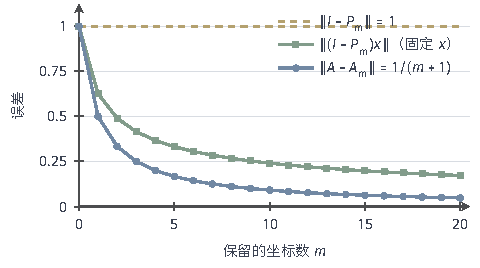
\includegraphics[width=81.2mm]{figures/02-abstract-mathematics/03-function-spaces/tikz/c3-finite-rank-error/figure.pdf}
  \caption{$\ell^2$上三种截断误差随保留坐标数$m$的变化。虚线：恒等算子的统一误差$\lVert I-P_m\rVert$恒为$1$。方点：固定单位向量$x\propto(1/n)$的误差$\lVert(I-P_m)x\rVert$趋于零，但这一速度只属于这个$x$。圆点：紧算子$A(x_n)=(x_n/n)$的统一误差$\lVert A-A_m\rVert=1/(m+1)$。}
  \label{fig:lop-finite-rank-error}
\end{figure}

\paragraph{紧算子的有限秩逼近}
现在证明反方向。思路是：紧算子的单位球像可以被有限个点以误差$\varepsilon$覆盖，这些点张成一个有限维子空间；向这个子空间作正交投影，就得到有限秩近似。正交投影的最近点性质保证投影误差不超过到覆盖点的距离。

\begin{theorem}[紧算子的有限秩逼近]
\label{thm:lop-finite-rank-approx}
设$X$是赋范空间，$H$是Hilbert空间，$T:X\to H$是紧算子。则存在有限秩算子$F_n:X\to H$，使$\lVert T-F_n\rVert\to0$。
\end{theorem}

\begin{proof}
给定$\varepsilon>0$。$T(B_X)$相对紧，因而全有界，取有限个点$y_1,\ldots,y_N$构成它的$\varepsilon$网。令$M=\operatorname{span}\{y_1,\ldots,y_N\}$，它是有限维子空间，因而闭；设$P$为到$M$的正交投影，令$F=PT$。$F$的像含于$M$，且$\lVert F\rVert\leq\lVert P\rVert\,\lVert T\rVert\leq\lVert T\rVert$，所以$F$是有界有限秩算子。

对任意$x\in B_X$，选$y_i$使$\lVert Tx-y_i\rVert<\varepsilon$。$PTx$是$M$中离$Tx$最近的点，而$y_i\in M$，所以
\[
\lVert Tx-Fx\rVert=\lVert Tx-PTx\rVert\leq\lVert Tx-y_i\rVert<\varepsilon .
\]
对$x\in B_X$取上确界得$\lVert T-F\rVert\leq\varepsilon$。令$\varepsilon=1/n$即得所需的算子列。
\end{proof}

这里控制的是整个单位球上的算子范数误差$\lVert T-F\rVert$，而不是只让$F$在有限几个输入上与$T$吻合；后者用强算子收敛就能做到，却不能保证统一误差。结合两个定理，在取值空间为Hilbert空间时，紧算子恰好是有界有限秩算子的算子范数极限。

证明真正用到的是Hilbert空间的正交投影：它把有限覆盖变成一个范数不超过$1$的线性“取最近点”操作。一般Banach空间中，有限维子空间上不一定有范数可控的投影族，紧算子能否由有限秩算子按算子范数逼近取决于空间的所谓逼近性质；确实存在不具有这一性质的Banach空间，这里不给出构造。所以本定理不能无条件推广，而定理~\ref{thm:lop-compact-limit}的方向在Banach空间中始终成立。

\subsection{积分算子的紧性}
\label{sec:lop-integral-compact}

沿用第~\ref{sec:lop-integral-bounded}小节的设定：$(X,\mu)$与$(Y,\nu)$是$\sigma$有限测度空间，$k\in L^2(X\times Y,\mu\otimes\nu)$，$T:L^2(Y,\nu)\to L^2(X,\mu)$由\eqref{eq:lop-integral-operator}给出。式\eqref{eq:lop-hs-norm}的估计对任意平方可积核成立，用于两个核之差就得到
\begin{equation}
\lVert T_k-T_{k^\prime}\rVert\leq\lVert k-k^\prime\rVert_{L^2(\mu\otimes\nu)},
\label{eq:lop-kernel-error}
\end{equation}
其中$T_k$表示以$k$为核的积分算子。所以只需用“给出有限秩算子的核”在$L^2$中逼近$k$，再用定理~\ref{thm:lop-compact-limit}。

\paragraph{分离变量的核给出有限秩算子}
若$k(x,y)=\sum_{i=1}^r\varphi_i(x)\psi_i(y)$，其中$\varphi_i\in L^2(\mu)$、$\psi_i\in L^2(\nu)$，则
\[
(Tf)(x)=\sum_{i=1}^r\Bigl(\int_Y\psi_i f\,\mathrm d\nu\Bigr)\varphi_i(x),
\]
输出落在$\operatorname{span}\{\varphi_1,\ldots,\varphi_r\}$中，$T$的秩不超过$r$。贯穿例子的核$1+xz=1\cdot1+x\cdot z$就是这样的有限和，所以\eqref{eq:lop-running-kernel}是秩为$2$的算子。最简单的分离变量核是可测矩形的示性函数$\mathbf 1_{A\times B}(x,y)=\mathbf 1_A(x)\mathbf 1_B(y)$，下面的引理说明它们的线性组合足以逼近任意可测集。

\begin{lemma}[矩形逼近]
\label{lem:lop-rectangle-approx}
设$(X,\mu)$、$(Y,\nu)$是有限测度空间，$E$属于乘积$\sigma$代数。则对每个$\varepsilon>0$，存在有限个两两不交的可测矩形，其并$R$满足$(\mu\otimes\nu)(E\,\triangle\,R)<\varepsilon$。
\end{lemma}

\begin{proof}
记$m=\mu\otimes\nu$，令$\mathcal E$为具有引理性质的可测集全体，$\mathcal R$为有限个两两不交可测矩形之并组成的族。两个矩形之交仍是矩形，矩形的补$(A\times B)^c=(A^c\times Y)\cup(A\times B^c)$是两个不交矩形之并，由此可知$\mathcal R$对有限交、补和有限并封闭。可测矩形显然属于$\mathcal E$。

若$E\in\mathcal E$，取$R\in\mathcal R$逼近它，则$R^c\in\mathcal R$且$E^c\triangle R^c=E\triangle R$，所以$\mathcal E$对补封闭。若$E_1,E_2,\ldots\in\mathcal E$，令$E=\bigcup_jE_j$。总测度有限，可取$N$使$m(E\setminus\bigcup_{j\leq N}E_j)<\varepsilon/2$；再对$j\leq N$取$R_j\in\mathcal R$使$m(E_j\triangle R_j)<\varepsilon/(2N)$。令$R=\bigcup_{j\leq N}R_j\in\mathcal R$，则
\[
m(E\triangle R)\leq m\Bigl(E\setminus\bigcup_{j\leq N}E_j\Bigr)+\sum_{j\leq N}m(E_j\triangle R_j)<\varepsilon .
\]
所以$\mathcal E$对可数并封闭。$\mathcal E$是包含全部可测矩形的$\sigma$代数，因而包含它们生成的乘积$\sigma$代数。
\end{proof}

\begin{theorem}[矩形阶梯核的稠密性]
\label{thm:lop-rectangle-dense}
形如
\begin{equation*}
\sum_{i=1}^rc_i\mathbf 1_{A_i}(x)\mathbf 1_{B_i}(y)\qquad(\mu(A_i),\nu(B_i)<\infty)
\end{equation*}
的函数在$L^2(X\times Y,\mu\otimes\nu)$中稠密。
\end{theorem}

\begin{proof}
第一步，截断到有限测度区域。由$\sigma$有限性，取递增的可测集$X_j\uparrow X$、$Y_j\uparrow Y$，且$\mu(X_j),\nu(Y_j)<\infty$。令$k_j=k\mathbf 1_{X_j\times Y_j}$，则$\lvert k-k_j\rvert^2\leq\lvert k\rvert^2$且逐点趋于零，由控制收敛定理$\lVert k-k_j\rVert_{L^2}\to0$。

第二步，用简单函数逼近。对$k_j$取简单函数$s_n\to k_j$逐点收敛且$\lvert s_n\rvert\leq\lvert k_j\rvert$（实部、虚部分别取单调逼近），则$\lvert k_j-s_n\rvert^2\leq4\lvert k_j\rvert^2$，由控制收敛定理$\lVert k_j-s_n\rVert_{L^2}\to0$。每个$s_n$是有限个$c_i\mathbf 1_{E_i}$之和，$E_i\subseteq X_j\times Y_j$可测。

第三步，用矩形代替可测集。在有限测度空间$X_j$与$Y_j$上应用引理~\ref{lem:lop-rectangle-approx}，每个$E_i$都可被有限个不交矩形之并$R_i$逼近，且$\lVert\mathbf 1_{E_i}-\mathbf 1_{R_i}\rVert_{L^2}=m(E_i\triangle R_i)^{1/2}$可任意小。三步的误差相加即得结论。
\end{proof}

\begin{theorem}[平方可积核给出紧算子]
\label{thm:lop-hs-compact}
在本小节的设定下，$T:L^2(Y,\nu)\to L^2(X,\mu)$是紧算子。
\end{theorem}

\begin{proof}
由定理~\ref{thm:lop-rectangle-dense}，对每个$\varepsilon>0$存在$k_\varepsilon(x,y)=\sum_{i=1}^rc_i\mathbf 1_{A_i}(x)\mathbf 1_{B_i}(y)$使$\lVert k-k_\varepsilon\rVert_{L^2}<\varepsilon$。$k_\varepsilon$是分离变量核，对应的积分算子把$f$送到$\sum_ic_i\bigl(\int_{B_i}f\,\mathrm d\nu\bigr)\mathbf 1_{A_i}$，是有限秩算子。由\eqref{eq:lop-kernel-error}，算子范数误差不超过$\varepsilon$。$L^2(X,\mu)$完备，由定理~\ref{thm:lop-compact-limit}，$T$是紧算子。
\end{proof}

证明中出现两种误差。$\lVert k-k_\varepsilon\rVert_{L^2(\mu\otimes\nu)}$度量的是两个核函数在乘积空间上的平方积分差，$\lVert T-T_{k_\varepsilon}\rVert$度量的是两个算子对单位输入的最坏输出差。式\eqref{eq:lop-kernel-error}只给出前者控制后者的单向关系；后者可以严格更小，正如贯穿例子中$\lVert T\rVert=1<\lVert k\rVert_{L^2}$。

图~\ref{fig:lop-rectangle-kernel}在贯穿例子上演示这一逼近。用$n\times n$网格上的格内平均作分片常数核$k_n$，它是$n^2$个矩形示性函数的线性组合，误差$\lVert k-k_n\rVert_{L^2}$大致按$1/n$下降。对这个核，分片常数逼近远不是最经济的：$k$本身的秩为$2$，两项就精确。矩形逼近的价值在于它对任意平方可积核都可行，从而在不知道核的任何具体结构时证明了紧性；按奇异值选取最经济的有限秩近似，是第~\ref{chap:operator-spectra}章的问题。

\begin{figure}[!htb]
  \centering
  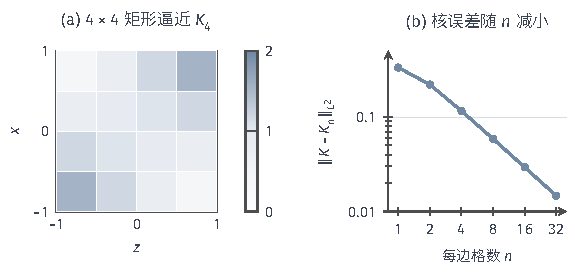
\includegraphics[width=97.4mm]{figures/02-abstract-mathematics/03-function-spaces/tikz/c3-rectangle-kernel/figure.pdf}
  \caption{用矩形示性函数的线性组合逼近核$k(x,z)=1+xz$（乘积测度由$\mathrm dz/2$给出）。(a)~$4\times4$均匀网格上取格内平均得到的分片常数核，每格对应一个可测矩形；(b)~$n\times n$网格平均的误差$\lVert k-k_n\rVert_{L^2}$，从$n=1$时的$1/3$降到$n=32$时约$0.015$，大致按$1/n$下降；它同时是相应有限秩算子的算子范数误差上界。}
  \label{fig:lop-rectangle-kernel}
\end{figure}

\section{完备空间中的基本算子定理}
\label{sec:lop-fundamental-theorems}

前面几节的估计都要求直接找到一个常数，控制单位球上的全部输入。实际问题中我们手里常常只有较弱的信息：每个固定输入上的输出有界；方程对每个右端都有唯一解；或者输入、输出同时收敛时极限相容。

对矩阵，这些信息已经足够，因为矩阵只有有限多列，每一列都有界就够了。无穷多列时，统一的常数要靠完备性来保证。三个定理都建立在第~\ref{chap:metric-spaces}章的Baire纲定理之上：完备度量空间不能写成可数个无内点闭集之并。

每个结论都要分别核对三件事：定义域是否完备，取值空间是否完备，算子是否定义在整个空间上。我们还要区分几种“好”的性质：逐输入有界与统一有界，代数上可逆（存在逆映射）与稳定可逆（逆映射有界）。

\subsection{一致有界原理}
\label{sec:lop-uniform-boundedness}

第~\ref{chap:linear-functionals}章对连续线性泛函族证明了：每个固定向量上的观测有界，整族的范数就有统一上界。这里把同样的论证用于取值于一般赋范空间的算子族，所得结论称为\term{一致有界原理}（uniform boundedness principle）。

\begin{theorem}[一致有界原理]
\label{thm:lop-uniform-boundedness}
设$X$是Banach空间，$Y$是赋范空间，$\{T_\alpha\}_{\alpha\in\Lambda}\subseteq\mathcal B(X,Y)$。若对每个$x\in X$都有$\sup_\alpha\lVert T_\alpha x\rVert<\infty$，则
\begin{equation}
 \sup_{\alpha\in\Lambda}\lVert T_\alpha\rVert<\infty.
 \label{eq:lop-uniform-boundedness}
\end{equation}
\end{theorem}

\begin{proof}
对$n\geq1$令
\[
 F_n=\{x\in X:\lVert T_\alpha x\rVert\leq n\text{ 对一切}\alpha\text{ 成立}\}.
\]
每个集合$\{x:\lVert T_\alpha x\rVert\leq n\}$是连续函数$x\mapsto\lVert T_\alpha x\rVert$的下水平集，因而闭；$F_n$是它们的交，也是闭集。由假设，每个$x$属于某个$F_n$，所以$X=\bigcup_nF_n$。

$X$完备，由Baire纲定理，某个$F_n$有内点：存在$x_0$与$r>0$使闭球$\overline B(x_0,r)\subseteq F_n$。对$\lVert z\rVert\leq r$，$x_0+z$与$x_0$都属于$F_n$，于是对一切$\alpha$，
\[
 \lVert T_\alpha z\rVert\leq\lVert T_\alpha(x_0+z)\rVert+\lVert T_\alpha x_0\rVert\leq2n .
\]
按线性缩放，$\lVert T_\alpha\rVert\leq2n/r$对一切$\alpha$成立。
\end{proof}

三个条件各司其职。算子的有界性使$F_n$闭；定义域的完备性通过Baire纲定理在某一层中找到一个球；线性把这个球平移到原点并缩放到单位球。取值空间的完备性没有用到。

定义域不完备时结论可以失败。令$X$为只有有限个非零项的序列全体，配$\ell^2$范数，它不完备。令$T_nx=nx_n$（取值于$\mathbb F$）。对每个$x\in X$，当$n$大于$x$最后一个非零项的位置时$T_nx=0$，所以$\sup_n\lvert T_nx\rvert<\infty$。

但$\lvert T_ne_n\rvert=n$，所以$\lVert T_n\rVert=n$无界。逐输入有界本身不是统一有界，二者之间的桥梁正是完备性。

\paragraph{强收敛极限的有界性}
一致有界原理回答了第~\ref{sec:lop-operator-convergence}节留下的问题。设$X$是Banach空间，$T_n\in\mathcal B(X,Y)$，且对每个$x$，$T_nx$在$Y$中收敛，记极限为$Tx$。收敛序列有界，所以$\sup_n\lVert T_nx\rVert<\infty$对每个$x$成立，由定理得
\[
 K=\sup_n\lVert T_n\rVert<\infty.
\]
于是$T$线性，并且
\[
 \lVert Tx\rVert=\lim_n\lVert T_nx\rVert\leq K\lVert x\rVert,
\]
$T$是有界算子。强算子收敛不能保证统一误差趋于零，却至少保证了统一的范数上界与极限的有界性。

\subsection{开映射定理}
\label{sec:lop-open-mapping}

由输出恢复输入，要同时满足三个要求：给定的输出有原像（存在），原像只有一个（唯一），输出上的小误差只造成输入上的小误差（稳定）。方阵可逆就同时满足这三条；无限维中它们会分离。

第~\ref{chap:topological-spaces}章把开集的像仍为开集的映射称为开映射，这与连续性要求的“开集的原像为开集”方向相反。对线性算子，开映射性质恰好给出逆向的误差估计，这就是下面的\term{开映射定理}（open mapping theorem）。

\begin{theorem}[开映射定理]
\label{thm:lop-open-mapping}
设$X,Y$是Banach空间，$T\in\mathcal B(X,Y)$是满射。则存在$\delta>0$使
\begin{equation}
 B_Y(0,\delta)\subseteq T(B_X(0,1)),
 \label{eq:lop-open-mapping}
\end{equation}
从而$T$是开映射。特别地，每个$y\in Y$都有原像$x$满足$\lVert x\rVert\leq2\delta^{-1}\lVert y\rVert$。
\end{theorem}

定理说的是：满射不仅保证每个输出都有原像，还保证能选到一个范数受控的原像。证明分两步：先用Baire纲定理得到输出球落在输入球之像的闭包中，再用逐步修正残差去掉闭包。

\begin{proof}
记$B_r=B_X(0,r)$。第一步，像的闭包含有输出球。由满射，
\[
 Y=\bigcup_kT(B_k)=\bigcup_k\overline{T(B_k)}.
\]
$Y$完备，由Baire纲定理，某个$\overline{T(B_k)}$含有开球$B_Y(y_0,\rho)$。对$\lVert y\rVert<\rho$，$y_0+y$与$y_0$都在$\overline{T(B_k)}$中，二者之差属于$\overline{T(B_k)-T(B_k)}\subseteq\overline{T(B_{2k})}$。

所以$B_Y(0,\rho)\subseteq\overline{T(B_{2k})}$。令$\eta=\rho/(2k)$，按线性缩放得
\[
 B_Y(0,\eta/2^j)\subseteq\overline{T(B_{2^{-j}})}\qquad(j\geq0).
\]

第二步，逐步修正残差。任取$\lVert y\rVert<\eta$。由第一步，存在$x_1\in B_1$使$\lVert y-Tx_1\rVert<\eta/2$。残差$y-Tx_1$落在$B_Y(0,\eta/2)$中，于是存在$x_2\in B_{1/2}$使$\lVert y-Tx_1-Tx_2\rVert<\eta/4$。如此继续，得到$x_j$满足
\[
 \lVert x_j\rVert<2^{1-j},\qquad\Bigl\lVert y-T\sum_{i\leq j}x_i\Bigr\rVert<\eta/2^j .
\]

第三步，用输入空间的完备性求和。$\sum_j\lVert x_j\rVert<2$，部分和是$X$中的柯西列；$X$完备，所以$x=\sum_jx_j$存在且$\lVert x\rVert<2$。由$T$连续，$Tx=y$。这说明$B_Y(0,\eta)\subseteq T(B_2)$，取$\delta=\eta/2$即得式~\eqref{eq:lop-open-mapping}。

第四步，验证开映射。设$U\subseteq X$开，$x\in U$，取$\varepsilon>0$使$B_X(x,\varepsilon)\subseteq U$。则
\[
 T(U)\supseteq Tx+\varepsilon T(B_1)\supseteq B_Y(Tx,\varepsilon\delta),
\]
所以$T(U)$开。

最后证明原像的估计。设$y\neq0$，$y^\prime=\delta y/(2\lVert y\rVert)$落在$B_Y(0,\delta)$中，由式~\eqref{eq:lop-open-mapping}有$x^\prime\in B_1$使$Tx^\prime=y^\prime$。令$x=2\lVert y\rVert x^\prime/\delta$，则$Tx=y$且$\lVert x\rVert\leq2\delta^{-1}\lVert y\rVert$。
\end{proof}

第一步只得到闭包：闭包中的点只能被像逼近，未必是像。第二步把“可以逼近”变成“可以达到”，代价是输入球的半径从$1$放大到$2$，并且必须用到$X$的完备性。图~\ref{fig:lop-open-mapping}用一个二维线性映射画出这个修正过程。

\begin{BookInlineFigure}
  \centering
  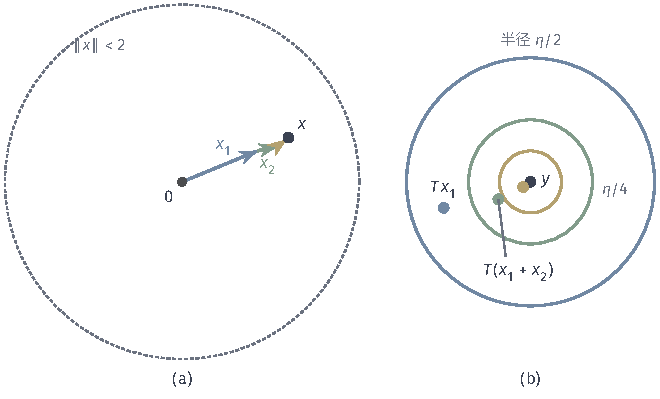
\includegraphics[width=111.725mm]{figures/04-spaces-measures-and-geometry/03-function-spaces/tikz/lop-open-mapping/figure.pdf}
  \caption{开映射定理证明中的残差修正，取$T=\operatorname{diag}(1,0.7)$，$\eta=1$作示意。(a)输入空间中修正量满足$\lVert x_j\rVert<2^{1-j}$，部分和收敛到原像$x$，$\lVert x\rVert<2$（虚线圆）。(b)输出空间中，近似$Tx_1$落在以$y$为心、半径$\eta/2$的圆内（蓝），加上修正后$T(x_1+x_2)$落入半径$\eta/4$的圆内（绿），第三次修正落入半径$\eta/8$的圆内（黄）。}
  \label{fig:lop-open-mapping}
\end{BookInlineFigure}

把开映射定理用于双射，原像的选取就是唯一的，于是逆映射自动连续。这一推论称为\term{有界逆定理}（bounded inverse theorem）。

\begin{theorem}[有界逆定理]
\label{thm:lop-bounded-inverse}
设$X,Y$是Banach空间，$T\in\mathcal B(X,Y)$是双射。则$T^{-1}\in\mathcal B(Y,X)$，并且
\begin{equation}
 \lVert T^{-1}\rVert\leq\delta^{-1},
 \label{eq:lop-bounded-inverse}
\end{equation}
其中$\delta$为开映射定理中的常数。
\end{theorem}

\begin{proof}
$T^{-1}$的线性来自$T$的线性。设$y\neq0$，$0<t<\delta$，由式~\eqref{eq:lop-open-mapping}，$ty/\lVert y\rVert$有原像落在$B_X(0,1)$中；$T$是单射，所以这个原像就是$T^{-1}(ty/\lVert y\rVert)$。于是
\[
 \lVert T^{-1}y\rVert<\frac{\lVert y\rVert}{t}.
\]
令$t\to\delta$，得$\lVert T^{-1}y\rVert\leq\delta^{-1}\lVert y\rVert$。
\end{proof}

\paragraph{代数可逆与稳定可逆}
有界逆定理说，在Banach空间之间，有界线性双射自动是稳定的：代数可逆就推出稳定可逆。条件不能省。$\ell^2$上的对角算子$A$是单射，它把$\ell^2$一一地映到像$\operatorname{Ran}A$上，在像上有逆映射$A^{-1}(y_n)=(ny_n)$。

这个逆相当于对角矩阵$\operatorname{diag}(1,2,3,\ldots)$，它无界：$\lVert A^{-1}e_n\rVert=n$，输出上$e_n/n$大小的误差会在恢复时变成长度为$1$的输入误差。原因在于$\operatorname{Ran}A$只是$\ell^2$中稠密而不闭的子空间（第~\ref{sec:lop-range-kernel}小节），按$\ell^2$范数不完备，定理的条件不成立。

开映射提供的正是局部误差估计：在原点附近半径$\delta$的输出球中，每个输出都有半径$1$以内的原像。线性把这一局部信息推广到所有尺度，就得到$\lVert T^{-1}y\rVert\leq\delta^{-1}\lVert y\rVert$。代数可逆只给出逆映射的存在；稳定可逆还要求这个统一的常数，二者在完备空间之间才自动重合。

\paragraph{两个完备范数的比较}
有界逆定理的一个直接用途是比较范数。设线性空间$X$在两个范数$\lVert\cdot\rVert_a$、$\lVert\cdot\rVert_b$下都完备，且$\lVert x\rVert_a\leq C\lVert x\rVert_b$。

恒等映射作为从$(X,\lVert\cdot\rVert_b)$到$(X,\lVert\cdot\rVert_a)$的映射是有界双射，其逆也有界，于是存在$C^\prime$使$\lVert x\rVert_b\leq C^\prime\lVert x\rVert_a$，两个范数等价。第~\ref{sec:lop-inclusions}节的$C[0,1]$上，$\lVert f\rVert_1\leq\lVert f\rVert_\infty$而两范数不等价，这与定理并不矛盾：$C[0,1]$在$\lVert\cdot\rVert_1$下不完备。

\subsection{闭图判别}
\label{sec:lop-closed-graph}

直接估计$\lVert Tx\rVert\leq C\lVert x\rVert$有时很困难。另一种思路是只检验一个较弱的条件：若输入$x_n\to x$，并且输出$Tx_n$也收敛到某个$y$，那么$y$是否必定等于$Tx$？这个条件不要求先证明输出收敛，只要求输入、输出同时收敛时极限相容。写成几何语言，就是算子的图
\begin{equation}
 \mathcal G(T)=\{(x,Tx):x\in D(T)\}\subseteq X\times Y
 \label{eq:lop-graph}
\end{equation}
在乘积范数$\lVert(x,y)\rVert=\lVert x\rVert+\lVert y\rVert$下是闭集。

$X,Y$都完备时，$X\times Y$也完备。下面的\term{闭图定理}（closed graph theorem）说明，对定义在整个完备空间上的算子，这个较弱的条件已经足够。

\begin{theorem}[闭图定理]
\label{thm:lop-closed-graph}
设$X,Y$是Banach空间，$T:X\to Y$是定义在整个$X$上的线性算子。则$T$有界当且仅当$\mathcal G(T)$在$X\times Y$中闭。
\end{theorem}

\begin{proof}
若$T$有界，$x_n\to x$推出$Tx_n\to Tx$，所以$Tx_n\to y$时$y=Tx$，图闭。

反过来，设图闭。它是Banach空间$X\times Y$的闭线性子空间，本身是Banach空间。第一坐标投影$\pi(x,Tx)=x$是从$\mathcal G(T)$到$X$的有界线性映射，因为$\lVert x\rVert\leq\lVert(x,Tx)\rVert$。它是双射，因为$T$定义在整个$X$上，每个$x$恰好对应图中一点。

由有界逆定理，$\pi^{-1}$有界：存在$C$使
\[
 \lVert x\rVert+\lVert Tx\rVert\leq C\lVert x\rVert,
\]
于是$\lVert Tx\rVert\leq C\lVert x\rVert$。
\end{proof}

图闭的条件同时考察输入与输出的极限：只知道$x_n\to x$而不知道$Tx_n$是否收敛，就无从检验；只看输出收敛而不管输入，也不能确定极限属于谁的图。定理的作用是把这个“两侧相容”的条件升级为有界性，代价是要求定义域为整个Banach空间。

\paragraph{处处有定义的对称算子有界}
设$T:H\to H$定义在整个Hilbert空间上，且$\langle v,Tx\rangle=\langle Tv,x\rangle$对一切$x,v$成立。若$x_n\to x$且$Tx_n\to w$，则对任意$v$，
\[
 \langle v,w\rangle=\lim_n\langle v,Tx_n\rangle=\lim_n\langle Tv,x_n\rangle=\langle Tv,x\rangle=\langle v,Tx\rangle ,
\]
所以$w=Tx$，图闭，$T$有界。这里没有估计任何范数，只用了对称性和内积的连续性。反过来说，无界的对称算子，例如适当定义域上的微分算子，不可能定义在整个Hilbert空间上。

\paragraph{定义域只是子空间时}
若$T$只定义在子空间$D(T)\subseteq X$上，图闭不再推出有界。回到求导$D:C^1[0,1]\subseteq C[0,1]\to C[0,1]$，两侧都用一致范数。它的图是闭的：若$f_n\to f$且$f_n^\prime\to g$都按一致范数，则在
\[
 f_n(x)=f_n(0)+\int_0^xf_n^\prime(t)\,\mathrm dt
\]
两边取极限，一致收敛允许在积分号下取极限，得到
\[
 f(x)=f(0)+\int_0^xg(t)\,\mathrm dt.
\]
所以$f\in C^1[0,1]$且$f^\prime=g$。

可是第~\ref{sec:lop-derivative-boundedness}小节已经用$\sin(2\pi nx)$说明$D$在一致范数下无界。两者不矛盾：$D(D)=C^1[0,1]$在一致范数下不完备，闭图定理的条件不满足。图闭的算子称为\term{闭算子}（closed operator）。

\paragraph{图范数}
对闭算子$T$，在定义域上换用\term{图范数}（graph norm）
\begin{equation}
 \lVert x\rVert_T=\lVert x\rVert_X+\lVert Tx\rVert_Y.
 \label{eq:lop-graph-norm}
\end{equation}
映射$x\mapsto(x,Tx)$把$(D(T),\lVert\cdot\rVert_T)$等距地映到图$\mathcal G(T)$上。当$X,Y$完备时，图作为闭子空间完备，所以$(D(T),\lVert\cdot\rVert_T)$是Banach空间，而$\lVert Tx\rVert_Y\leq\lVert x\rVert_T$说明$T$在新范数下有界。

对求导，图范数正是$\lVert f\rVert_{C^1}$。这就兑现了第~\ref{sec:lop-derivative-boundedness}小节的说法：配上$C^1$范数后定义域完备，同一个作用规则成为Banach空间之间的有界算子。

因此，把基本定理用于定义在真子空间上的算子之前，必须先确认所用的范数使定义域完备。第~\ref{chap:sobolev-spaces}章的Sobolev范数沿用同样的思想，用积分范数同时控制函数和它的弱导数。

\section{本章小结}
\label{sec:lop-summary}

本章把函数到函数的变换写成线性算子，并始终把定义域、取值空间和两侧的范数当作算子的一部分。恒等、投影与乘以有界函数自然定义在整个空间上；积分公式要由核、测度与输入空间共同保证有意义；求导只能定义在可导函数组成的真子空间上。说一个算子“有界”，就是说存在统一常数$C$使$\lVert Tx\rVert\leq C\lVert x\rVert$；对线性算子，这等价于连续与Lipschitz连续，最小的这种常数就是算子范数，它统一控制输入差造成的输出差。

同一个公式在不同范数下可以有完全不同的行为。求导在一致范数下无界，在$C^1$范数下有界；平方可积核给出有界积分算子，且$\lVert T\rVert\leq\lVert k\rVert_{L^2}$。包含映射把“同一个函数在不同空间中的大小”变成算子的有界性：有限测度上$L^q$连续嵌入$L^p$（$p\leq q$），计数测度上方向相反；改变测度时先由绝对连续性保证等价类的对应，再由密度的上下界决定有界性与范数等价。算子列的范数收敛给出统一误差，强算子收敛只给出逐输入误差，截断投影说明两者确实不同。

Hilbert空间中，伴随把输出方向拉回输入空间，给出$(\operatorname{Ran}T)^\perp=\ker T^*$与$\overline{\operatorname{Ran}T}=(\ker T^*)^\perp$；像未必闭，与$\ker T^*$正交的输出只能被逼近，未必真正可达。自伴是同一空间上$T=T^*$的附加结构，正性还要求二次型非负，二者都不能由核在个别点上的符号判断。紧算子把有界输入列变成有收敛子列的输出列，把弱收敛改善为范数收敛；在Hilbert空间中它们恰好是有限秩算子的算子范数极限，平方可积核的积分算子都是紧算子，核的$L^2$误差控制算子范数误差。

完备性把较弱的信息升级为统一控制：一致有界原理由逐输入有界得到统一的范数上界，开映射定理与有界逆定理由满射与双射得到稳定的逆，闭图定理由图的闭性得到有界性。这些结论都需要定义域与取值空间完备，定义在真子空间上的算子须先换用使定义域完备的图范数。第~\ref{chap:operator-spectra}章在这些基础上研究$T-\lambda I$何时可逆，并为紧自伴算子与一般紧算子建立特征展开和奇异分解；给定输出求解算子方程的可解性与稳定性，留到第~\ref{chap:linear-operator-equations}章。

